\chapter{\label{par_est}Parameter estimation using SOAP}
%%%%%%%%%%%%
%%%%%%%%%%%%
%%%%%%%%%%%%
%%%%%

Throughout Chapters \ref{soap} and \ref{machine} we have developed
techniques that could identify whether a potential \gls{CW}
signal is present within a small frequency band of width $0.1$ Hz, and then
return the frequency track that the signal is most likely to follow.  This
provides the frequency bands in which a signal could be present, which is useful
for all-sky searches as it can limit the parameter space and therefore
computational time for deeper searches such as those described in
Sec.~\ref{searchcw:search:targeted}.  However, this only limits the parameter
space in frequency to a smaller frequency band, where there is still a large
parameter space which needs to be searched.  If the Viterbi track returned by
SOAP in Chapter \ref{soap} follows the frequency evolution of a \gls{CW}
source, then this track contains information on the sky position and frequency
evolution of the \gls{CW}.  If one could extract this information then the size
of the parameter space could be reduced for more sensitive coherent searches, decreasing their computational cost.

In this chapter I will outline a Bayesian method that uses the output Viterbi tracks of the SOAP search in Chapter~\ref{soap} to return a subset of astrophysical parameters of a
source.  Section~\ref{par_est:freq} will outline the model of the frequency
evolution of a \gls{CW} from a source with a slowly varying frequency,
Sec.~\ref{par_est:bayes} will outline the Bayesian model for this analysis and
Sec.~\ref{par_est:results} will show the results from testing on simulated
signals.

%%%%
%%%%
\section{\label{par_est:freq}\gls{CW} source frequency evolution}
%%%%
%%%%

The SOAP search, both single and multi detector, returns a frequency track known as the Viterbi track, if this
track follows the frequency of a \gls{CW} source, then the frequency evolution
contains information of the sky position ($\alpha, \delta$), the frequency of
the source $f$ and its derivative $\dot{f}$, where we ignore higher order
frequency derivatives.  From the Viterbi track, we should then be able to
extract this information as we have a model for the phase evolution (and
therefore frequency evolution) of the source described in
Eq.~\ref{searchcw:model:phase} in Sec.~\ref{searchcw:model}.  To relate this
phase evolution to the sky position parameters, we can look closer at
Eq.~\ref{searchcw:model:ssbtime}, where we describe the shift in arrival time
due to the Earth's motion.

The second term in Eq.~\ref{searchcw:model:ssbtime} describes the Doppler shift
due to the earth's orbit and rotation.  Where the $\bm{r}$ is the position of
the detector and $\bm{n}$ is a unit vector in the direction of the source.  As
in \citep{schutz1998DataAnalysis}, we use the ecliptic coordinate frame in the \gls{SSB}
where the $z$ axis is perpendicular to the ecliptic and the $x$ axis points towards the first point of Aries.  In this frame the unit vector pointing
towards the source can be written as
%
\begin{equation}
    \label{par_est:freq:unit}
    \bm{n} = 
    \left(
    \begin{matrix}
        1 & 0 & 0  \\
        0 & \cos \epsilon & \sin \epsilon \\
        0 & -\sin \epsilon & \cos \epsilon \\
    \end{matrix} \right)
    \left(
    \begin{matrix}
        \cos(\alpha)\cos(\delta)  \\
        \sin(\alpha)\cos(\delta) \\
        \sin(\delta) \\
    \end{matrix} \right),
\end{equation}
%
where $\alpha$ and $\delta$ are the right ascension and declination (sky
position) of the source and $\epsilon$ is the obliquity of the ecliptic, which is the inclination angle of the earths equator with respect to the ecliptic.  The first matrix in Eq.~\ref{par_est:freq:unit} describes
a rotation from the celestial frame to
the ecliptic frame an the second vector transforms the sky position parameters to their component $x,y,z$ coordinates in the celestial frame.

The position vector of the detector,
$\bm{r}$ in Eq.~\ref{searchcw:model:ssbtime}, at a time $t$ can be split into two components,
the position due to the orbit of the earth and position due to the rotation of
the detector.
If we assume the orbit is circular, then the position of the earth in its orbit
is described in Cartesian coordinates as
%
\begin{equation}
    \bm{r}_{\rm{orb}} = R_{\mathrm{orb}}
    \left(
    \begin{matrix}
        \cos{\left( \Omega_{\mathrm{orb}} t   \right)}  \\
        \sin{\left( \Omega_{\mathrm{orb}} t   \right)} \\
        0 \\
    \end{matrix} \right),
\end{equation}
%
where $R_{\mathrm{orb}}$ is the radius of the earth's orbit (1 AU),
$\Omega_{\mathrm{orb}}$ is the angular frequency of the earth's orbit
$2\pi/T_{\mathrm{orb}}$, where $T_{\mathrm{orb}}$ is one year and the time $t=0$ is when the earth is at the spring equinox.  The
position due to the rotation of the earth can then be described by 
%
\begin{equation}
    \bm{r}_{\rm{rot}} = R_{\mathrm{rot}}
    \left(
    \begin{matrix}
        1 & 0 & 0  \\
        0 & \cos \epsilon & \sin \epsilon \\
        0 & -\sin \epsilon & \cos \epsilon \\
    \end{matrix} \right)
    \left(
    \begin{matrix}
        \cos{(\beta)}\cos{\left( \Omega_{\mathrm{rot}} t + \phi_{\mathrm{rot}}  \right)}  \\
        \cos{(\beta)}\sin{\left( \Omega_{\mathrm{rot}} t + \phi_{\mathrm{rot}}  \right)} \\
        \sin{(\beta)} \\
    \end{matrix} \right),
\end{equation}
%
where $R_{\mathrm{rot}}$ is the radius of the earth, $\Omega_{\mathrm{rot}}$ is the
angular frequency of the earth's rotation $2\pi/T_{\mathrm{R}}$, where
$T_{\mathrm{rot}}$ is one day and $\beta$ is the detectors latitude. The phase $\phi_{\mathrm{rot}}$ defines the position of the earth in its rotation at $t=0$ and is determined by $\phi_{\mathrm{rot}} = \rm{LST}_{t=0} = \rm{GMST}_{t=0} - \lambda$, where $\lambda$  is the longitude of
the detectors site, the \gls{GMST} is the angle between the first point of Aries and the Greenwich meridian and the LST is the local sidereal time. The sum of these two components
then define the location of the detector in the \gls{SSB} frame
%
\begin{equation}
    \bm{r} = \bm{r}_{\rm{orb}} + \bm{r}_{\rm{rot}}.
\end{equation}

We can now describe the phase evolution of the signal at the detector
sites (latitude $\beta$ and longitude $\lambda$) starting at a time $t=0$ from the source sky
position ($\alpha, \delta$), frequency$f$ and its derivative
$\dot{f}$.  We can write the phase evolution from Eq.~\ref{searchcw:model:phase} as
%
\begin{equation}
    \label{par_est:freq:ph_evolution}
    \begin{split}
        \Phi(t) = 2\pi \left(  f_0 t + \frac{\dot{f} t^2}{2} \right) &+ \frac{2\pi}{c} \left(  f_0 + \dot{f}t  \right) \left\{ R_{\rm{orb}} \left[ \cos \alpha \cos \delta \cos \left( \Omega_{\mathrm{orb}} t \right) \right. \right. \\ 
        &+ \left. \left( \cos \epsilon \cos \alpha \cos \delta +  \sin \epsilon \sin \delta \right) \sin \left( \Omega_{\mathrm{orb}} t  \right) \right] \\
        &+ \left. R_{\rm{rot}} \left[ \sin \beta \sin \delta + \cos \beta \cos \delta \cos \left( \alpha - \Omega_{\mathrm{rot}} t - \phi_{rot}  \right)     \right] \right\},
    \end{split}
\end{equation}
%
where we ignore frequency derivatives higher than first order.
The frequency of a \gls{CW} signal at any point on the frequency track is then defined by the derivative of
the phase with respect to the detector time
%
\begin{equation}
f(t) = \frac{1}{2\pi}\frac{d\Phi(t)}{dt}.
\end{equation}
%.

%
%
\section{\label{par_est:bayes}Bayesian Model}
%
%

As described in Sec.~\ref{par_est:freq} we have a model of the frequency
evolution of a \gls{CW} and we have a Viterbi track which is our observation of
a frequency track.  We would now like to estimate the parameters $\bm{\theta} =
\left\{\alpha, \delta, f, \dot{f} \right\}$ of a \gls{CW} given that we have
observed the frequency track $\bm{V}$.  To do this we use a Bayesian model
%
\begin{equation}
    \label{par_est:bayes:eqn}
    p(\bm{\theta} \mid \bm{V}, I) = \frac{p(\bm{\theta} \mid I) p(\bm{V} \mid \bm{\theta}, I)}{p(\bm{V} \mid I)}
\end{equation}
%
where $p(\bm{\theta} \mid \bm{V}, I)$ is the posterior which we are interested in,
$p(\bm{\theta})$ is the prior, $p(\bm{V} \mid \bm{\theta}, I)$ is the
likelihood and $p(\bm{V} \mid I)$ is the Bayesian Evidence. The
following sections will describe how we define the prior and likelihood for
this problem.

%
%
\subsection{\label{par_est:bayes:likelihood}Likelihood}
%
%

The likelihood describes the probability of measuring the data
given a signal, where in this case our data is the Viterbi track $\bm{V}$ and
our signal is the model frequency track $\bm{M}(\bm{\theta})$.  The aim is to
find this probability distribution such that we can evaluate it for any model
parameters $\bm{\theta}$ and any data $\bm{V}$.

We define our likelihood from the deviation in frequency bins of the Viterbi
track from a model frequency track given some parameters $\bm{\theta}$, i.e.
$\bm{M}(\bm{\theta}) - \bm{V}$.  If the simulated \gls{CW} signal has an
infinitely large \gls{SNR} then the Viterbi track would follow the \gls{CW}
frequency track exactly, giving a delta function with 0 variance for the
deviation of the Viterbi and \gls{CW} frequency tracks. If conversely, the \gls{SNR} was zero
then the Viterbi track would wander randomly through the frequency band
independently of the \glspl{CW} frequency track, meaning that the deviation of
the two frequency tracks would have a variance $\mathcal{O}(\text{width})$
width of the
frequency band.  The distribution of these deviations is then dependent on the
\gls{SNR} $\rho$ of the signal.  

We can also think about how the Viterbi track will deviate from the model frequency track for different values of the parameters $\bm{\theta}$.
For a fixed \gls{SNR} we assume that the deviation of the two tracks is independent of the parameters which define the frequency evolution of the signal. 
For simplicity, we also assume that the deviation of the tracks is independent of the track position.
Given that the distribution of the deviations is difficult to find analytically, we calculate it empirically using the deviations of the two frequency tracks for many simulated of \gls{CW} signals. 

In Sec.~\ref{machine:results} we generated $\mathcal{O}(10^{4})$ simulated
\gls{CW} signals in Gaussian noise between 40 and 500 Hz, which had \gls{SNR}
$\rho$ uniformly distributed between 40 and 200 and
source parameters which follow those in
Tab.~\ref{machine:data:injections:table}. For each of these simulations, the
SOAP search using the line-aware statistic with parameters from
Sec.~\ref{soap:results} returns a Viterbi track associated with the simulated
parameters.  As we have assumed the distribution of the deviations is independent of the position in the track, we can calculate the difference between the Viterbi track and simulated \gls{CW} frequency track $M_i(\bm{\theta}^{\rm{sim}}) - V_i$ for each
element in the track and each simulation .
At a fixed \gls{SNR}, the density of these at a given deviation is the likelihood $\mathcal{L}$. 
We can model the likelihood distribution by finding the histogram of the track deviations.  As the track deviations are
integer frequency bin widths, the histogram bins centers are at $0, \pm 1, \pm 2 .... \pm W$, where $W$ is the width of the frequency band
in bins.

In this case our likelihood is also dependent on \gls{SNR}, therefore, we split
our simulations into bins of width \gls{SNR} 2 between 40 and 200. Within each
\gls{SNR} bin, this gives us $\sim 300$ simulated tracks each with $\sim 400$
elements.  In Fig.~\ref{par_est:bayes:likelihood:kde142}, rather than using a histogram we use a \gls{KDE}, which is a different method to estimate the probability density, this is the same result but makes the likelihood easier to interpret in a plot. Figure \ref{par_est:bayes:likelihood:kde142} shows an example of the \glspl{KDE} for a subset of the \gls{SNR} bins. The sharp peaks in the center of
each \gls{KDE} in Fig.~\ref{par_est:bayes:likelihood:kde142} represent
simulations where the Viterbi track is close to the simulated \gls{CW} track,
and the broader distributions represent areas where the Viterbi track has not
identified the \gls{CW} track but is wandering randomly.
Figure \ref{par_est:bayes:likelihood:kde142} shows that as the \gls{SNR}
increases, the distribution is more closely centred around 0, i.e. the Viterbi
and \gls{CW} tracks are similar, which is expected.

%
\begin{figure}[ht]
    \centering
    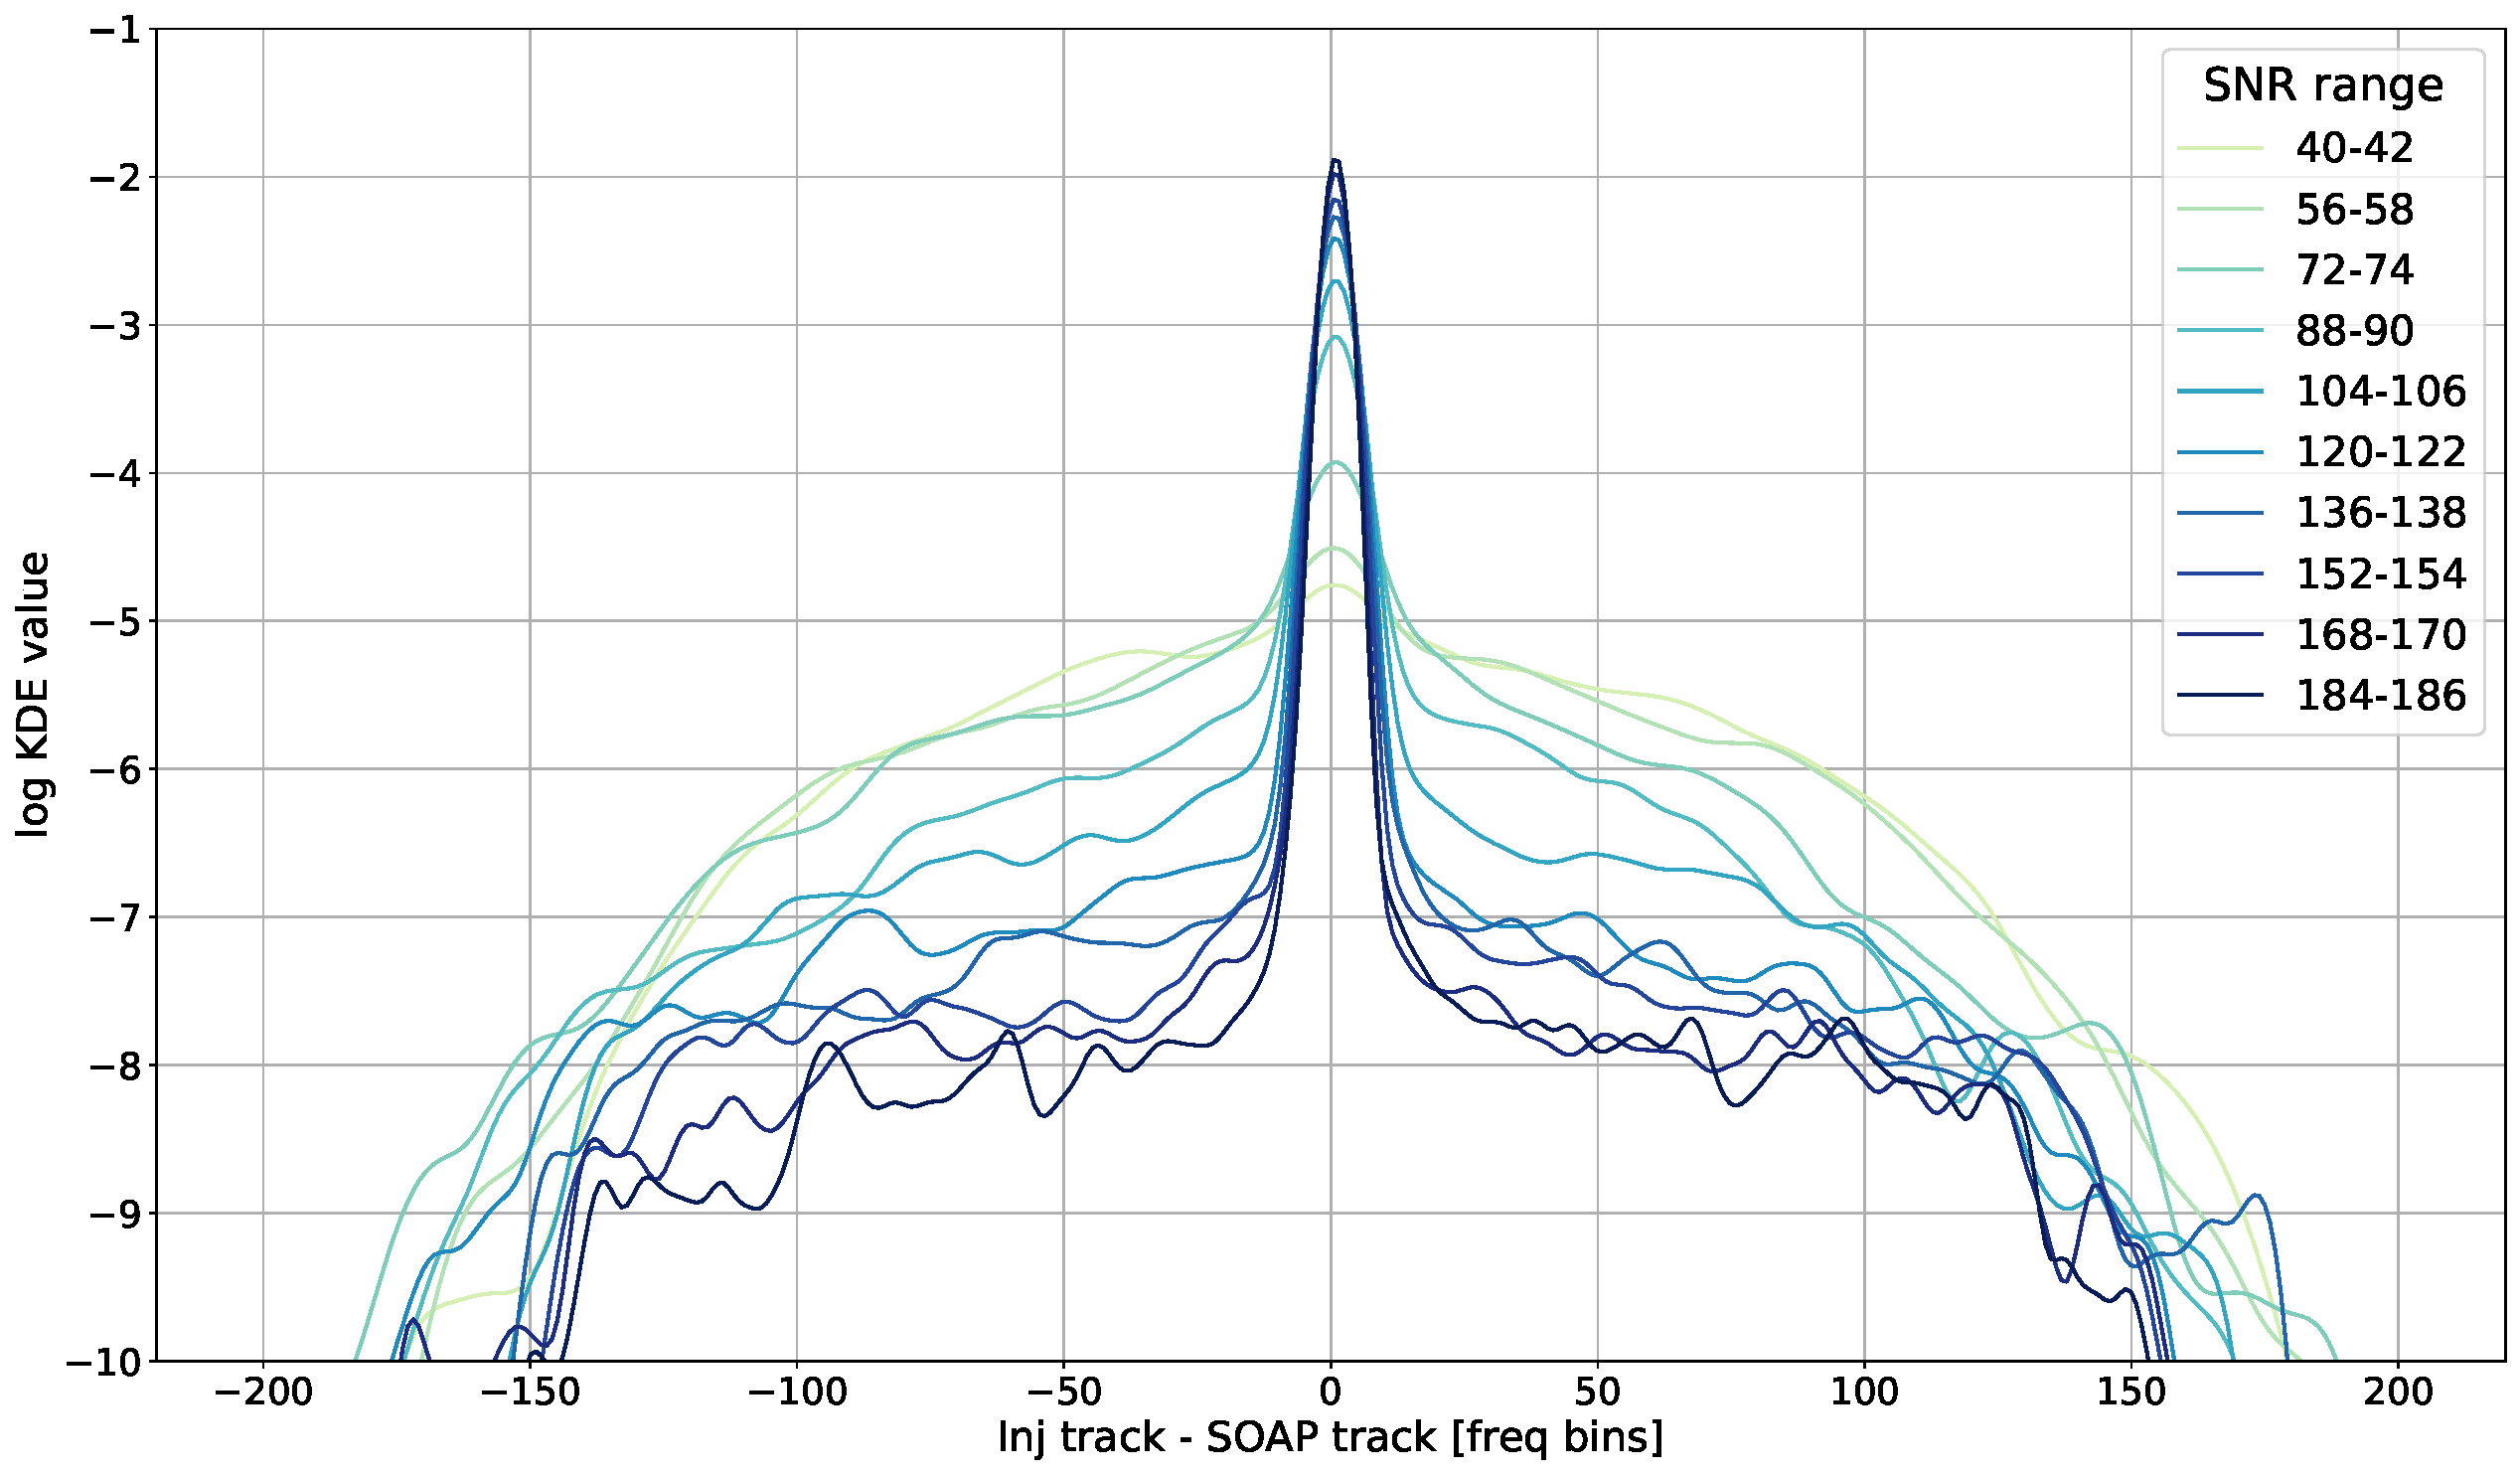
\includegraphics[width=\linewidth]{C5_parameter/KDE_range_40_200.pdf}
    \caption[KDE of likelihood in different \gls{SNR} ranges]{The likelihood can be modelled by using an \gls{KDE} or a histogram. Here we show the \gls{KDE} of the deviation of the recovered Viterbi track from
the simulated (injected) \gls{CW} frequency track for a number of \gls{SNR} ranges. The deviation of the track is
measured in discrete frequency bins. Each \gls{KDE} is generated from $\sim
300$ simulations which each have $\sim 400$ elements in their frequency tracks.
This shows a subset of the binned likelihoods between the range of \gls{SNR} 40
and 200.} \label{par_est:bayes:likelihood:kde142}
    \end{figure}
%

The dependence of the likelihood on the \gls{SNR} $\rho$ introduces one more parameter
to include in our Bayesian model.  
The likelihood is binned in \gls{SNR} with widths of $\rho_w = 2$ as described above, therefore any value of $\rho$ which lies in the range $\rho_c \pm \rho_w/2 $ uses the likelihood \gls{KDE} $\mathcal{L}_{\rho_c}$, where $\rho_c$ is the bin center.
The \glspl{KDE} $\mathcal{L}_{\rho_c}$ are then used to define the likelihood function $p(\bm{V} \mid
\bm{\theta}, \rho, I)$ in Eq.~\ref{par_est:bayes:eqn}, where we now have five parameters in our model
$\alpha, \delta, f, \dot{f}$ and $\rho$.  As we assume
independent track elements for a given Viterbi track, the likelihood is then the product of the likelihoods at each track element
%
\begin{equation} 
p(\bm{V} \mid \bm{\theta}, \rho, I) = \prod_{i =
1}^{N} \mathcal{L}_{\rho_c(\rho)}(M_i(\bm{\theta}) - V_i) , 
\end{equation} 
%
where $N$ is the length of the Viterbi track $\bm{V}$. 

% Not currently doing this 
\if
As the likelihood $\mathcal{L}$ is binned in \gls{SNR} $\rho$, and $\rho$ is a
continuous value, the likelihood is calculated as the weighted sum of the
surrounding likelihood bins, where the weights are the fractional separation of
$\rho$ from the bin centers.  
\fi

%
\subsection{Prior}
%
For this analysis we choose to use a simple prior which is flat in parameter space in some range.  We use a flat prior for $\alpha$
between $[0,2\pi]$, a flat prior in $\sin{\delta}$ between [-1,1], a flat prior
in $f$ in the range of the 0.1 Hz wide sub-band which SOAP searched through, a
flat prior in the frequency derivative in the range
$[-10^{-9},10^{-9}]$ Hz/s and a flat prior for the \gls{SNR} $\rho$ in
the range $[40,200]$.


%%%%
%%%%
\section{\label{par_est:results}Results}
%%%%
%%%%

The method described in Sec.~\ref{par_est:bayes} takes in a Viterbi track and
uses this to estimate the five dimensional posterior distribution
$p\left(\left\{ \alpha, \delta, f, \dot{f}, \rho \right\} \mid \bm{V}, I
\right)$.  To calculate this posterior we use a technique known as nested
sampling, specifically the package {\it Dynesty}
\citep{speagle2019DynestyDynamic}, which is introduced in
Sec.~\ref{searchcw:prob:bayes:nested}.

As an example of what the Bayesian analysis returns, we can first simulate a \gls{CW} signal with
parameters 
%
\begin{equation}
    \label{par_est:results:examplepars}
    \begin{split}
        \alpha &= 4.2 \; \rm{rad}\\
        \delta &= -0.06 \; \rm{rad} \\
        f &= 148.23 \; \rm{Hz}\\
        \dot{f} &= -3.55 \times 10^{-15} \; \rm{Hz/s} \\
        \rho &= 151,\\
    \end{split}
\end{equation}
%
and generate the associated spectrograms for the \gls{LIGO} detectors H1 and
L1 shown in Fig.~\ref{par_est:results:freqtrack}. The SOAP search from
Chapter \ref{soap} is then run using the line-aware statistic with the same
parameters as given in Tab.~\ref{soap:results:parameters}, where the multi detector search returns a single frequency track. The output Viterbi track is then plotted with the \gls{CW} frequency track in Fig.~\ref{par_est:results:freqtrack}. 
%
\begin{figure}[ht]
    \centering
    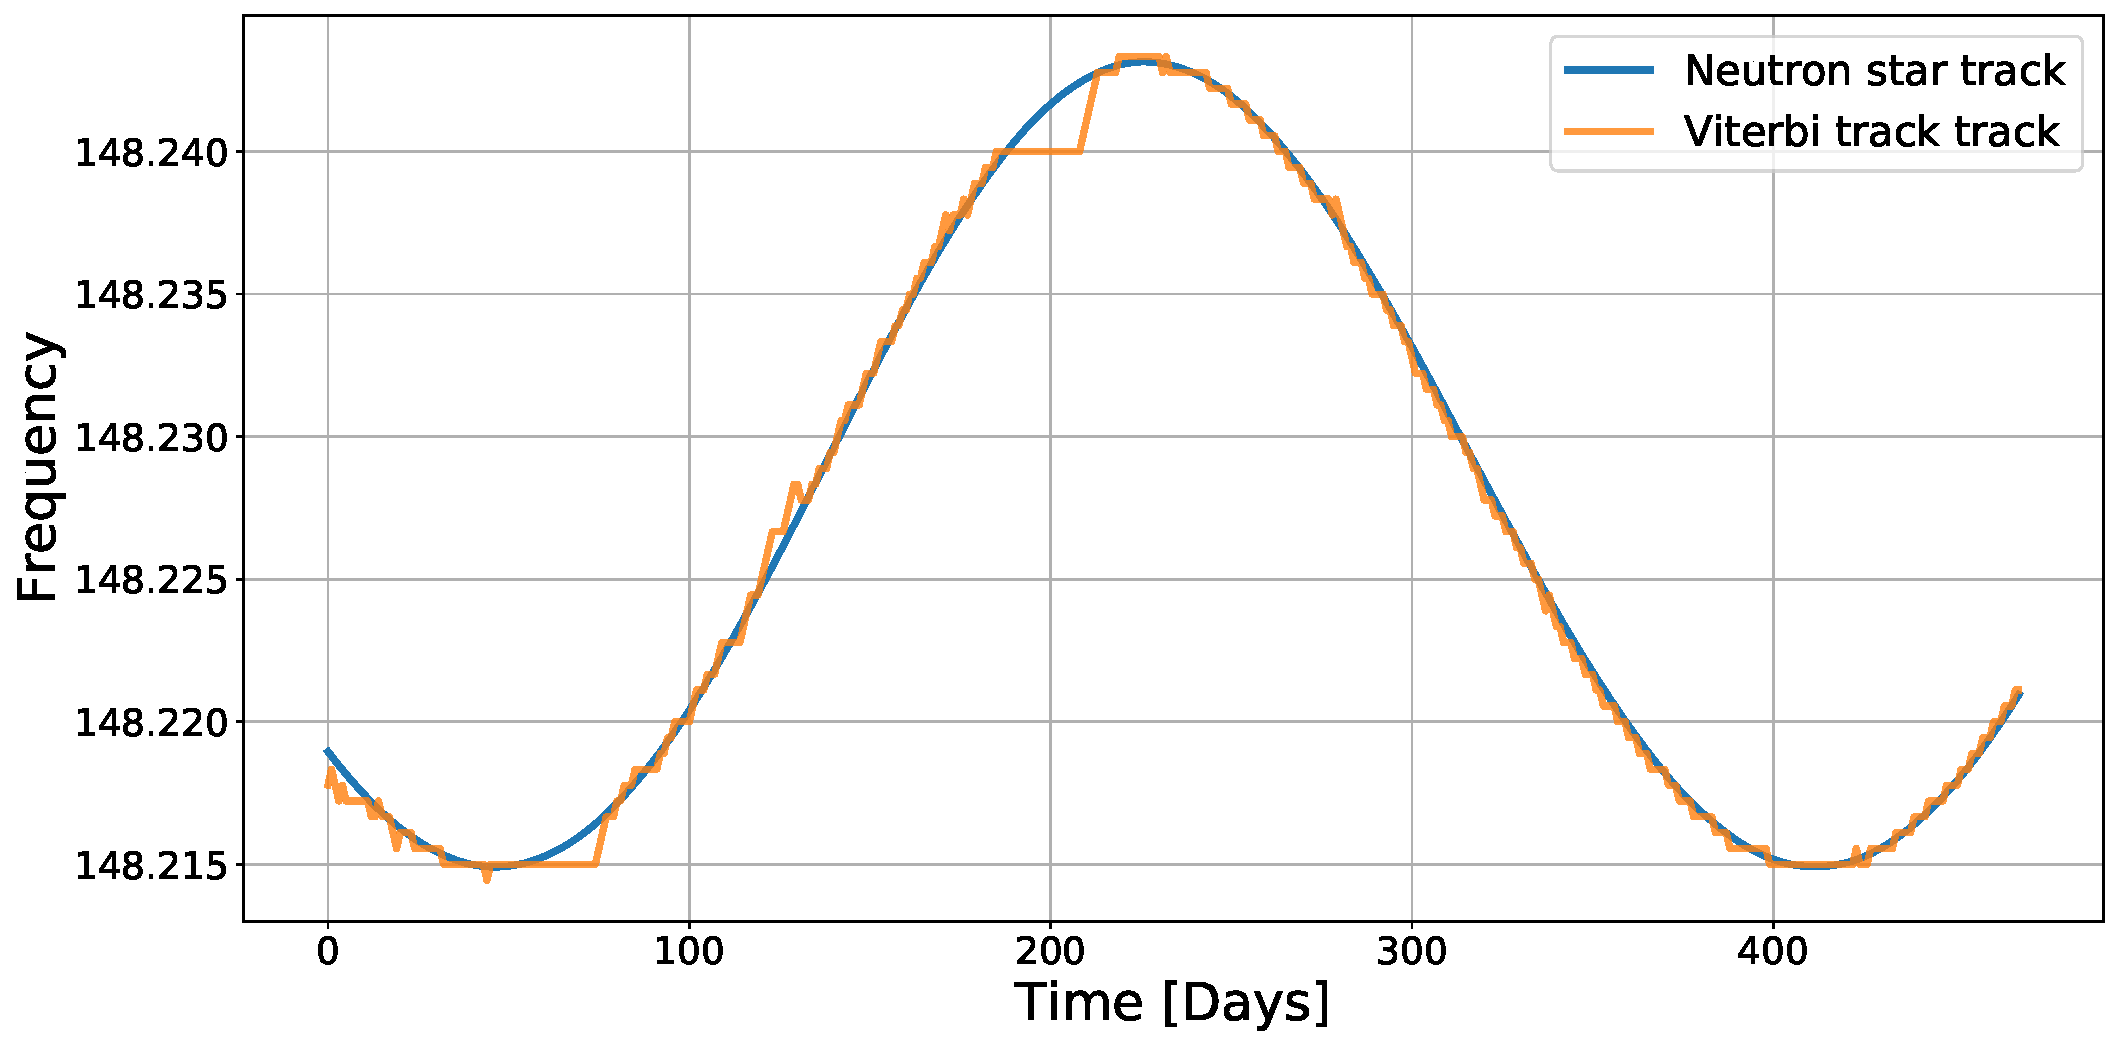
\includegraphics[width=\linewidth]{C5_parameter/example_freqtrack.pdf}
    \caption[Frequency track of injected signal]{ Example simulated \gls{CW} simulation in \gls{LIGO} detectors H1 and L1 using parameters in Eq.~\ref{par_est:results:examplepars}. The simulated frequency track of the signal is shown as the black line. The multi detector analysis returns a single frequency track (Viterbi track) which is the red line shown overlaid in both detectors.
    Both the Viterbi track and the simulated frequency track are shifted up in frequency bu 0.01 Hz to make the signal visible in the spectrogram.
    The track is sampled once per day, where the oscillation visible here is due to the Doppler modulation of the Earth's orbit.} \label{par_est:results:freqtrack}    
\end{figure}
%
In this case the Viterbi track can be seen to closely follow the simulated
\gls{CW} frequency track.

The Bayesian analysis described in Sec.~\ref{par_est:bayes} is then run using
this Viterbi track as input, where this returns the posterior distribution
shown in Fig.~\ref{par_est:results:example_posterior}.  In this example, the
injected parameter values (marked in orange) are contained within the marginal
posterior distributions for all of the parameters excluding the \gls{SNR}.  The
distribution in \gls{SNR} appears to have hard edges at the edge of the binned
likelihood function, which begins to demonstrate some problems with the
definition of the likelihood, this will described more in Sec.~\ref{par_est:results:simulations}.
%
\begin{figure}[pt]
    \centering
    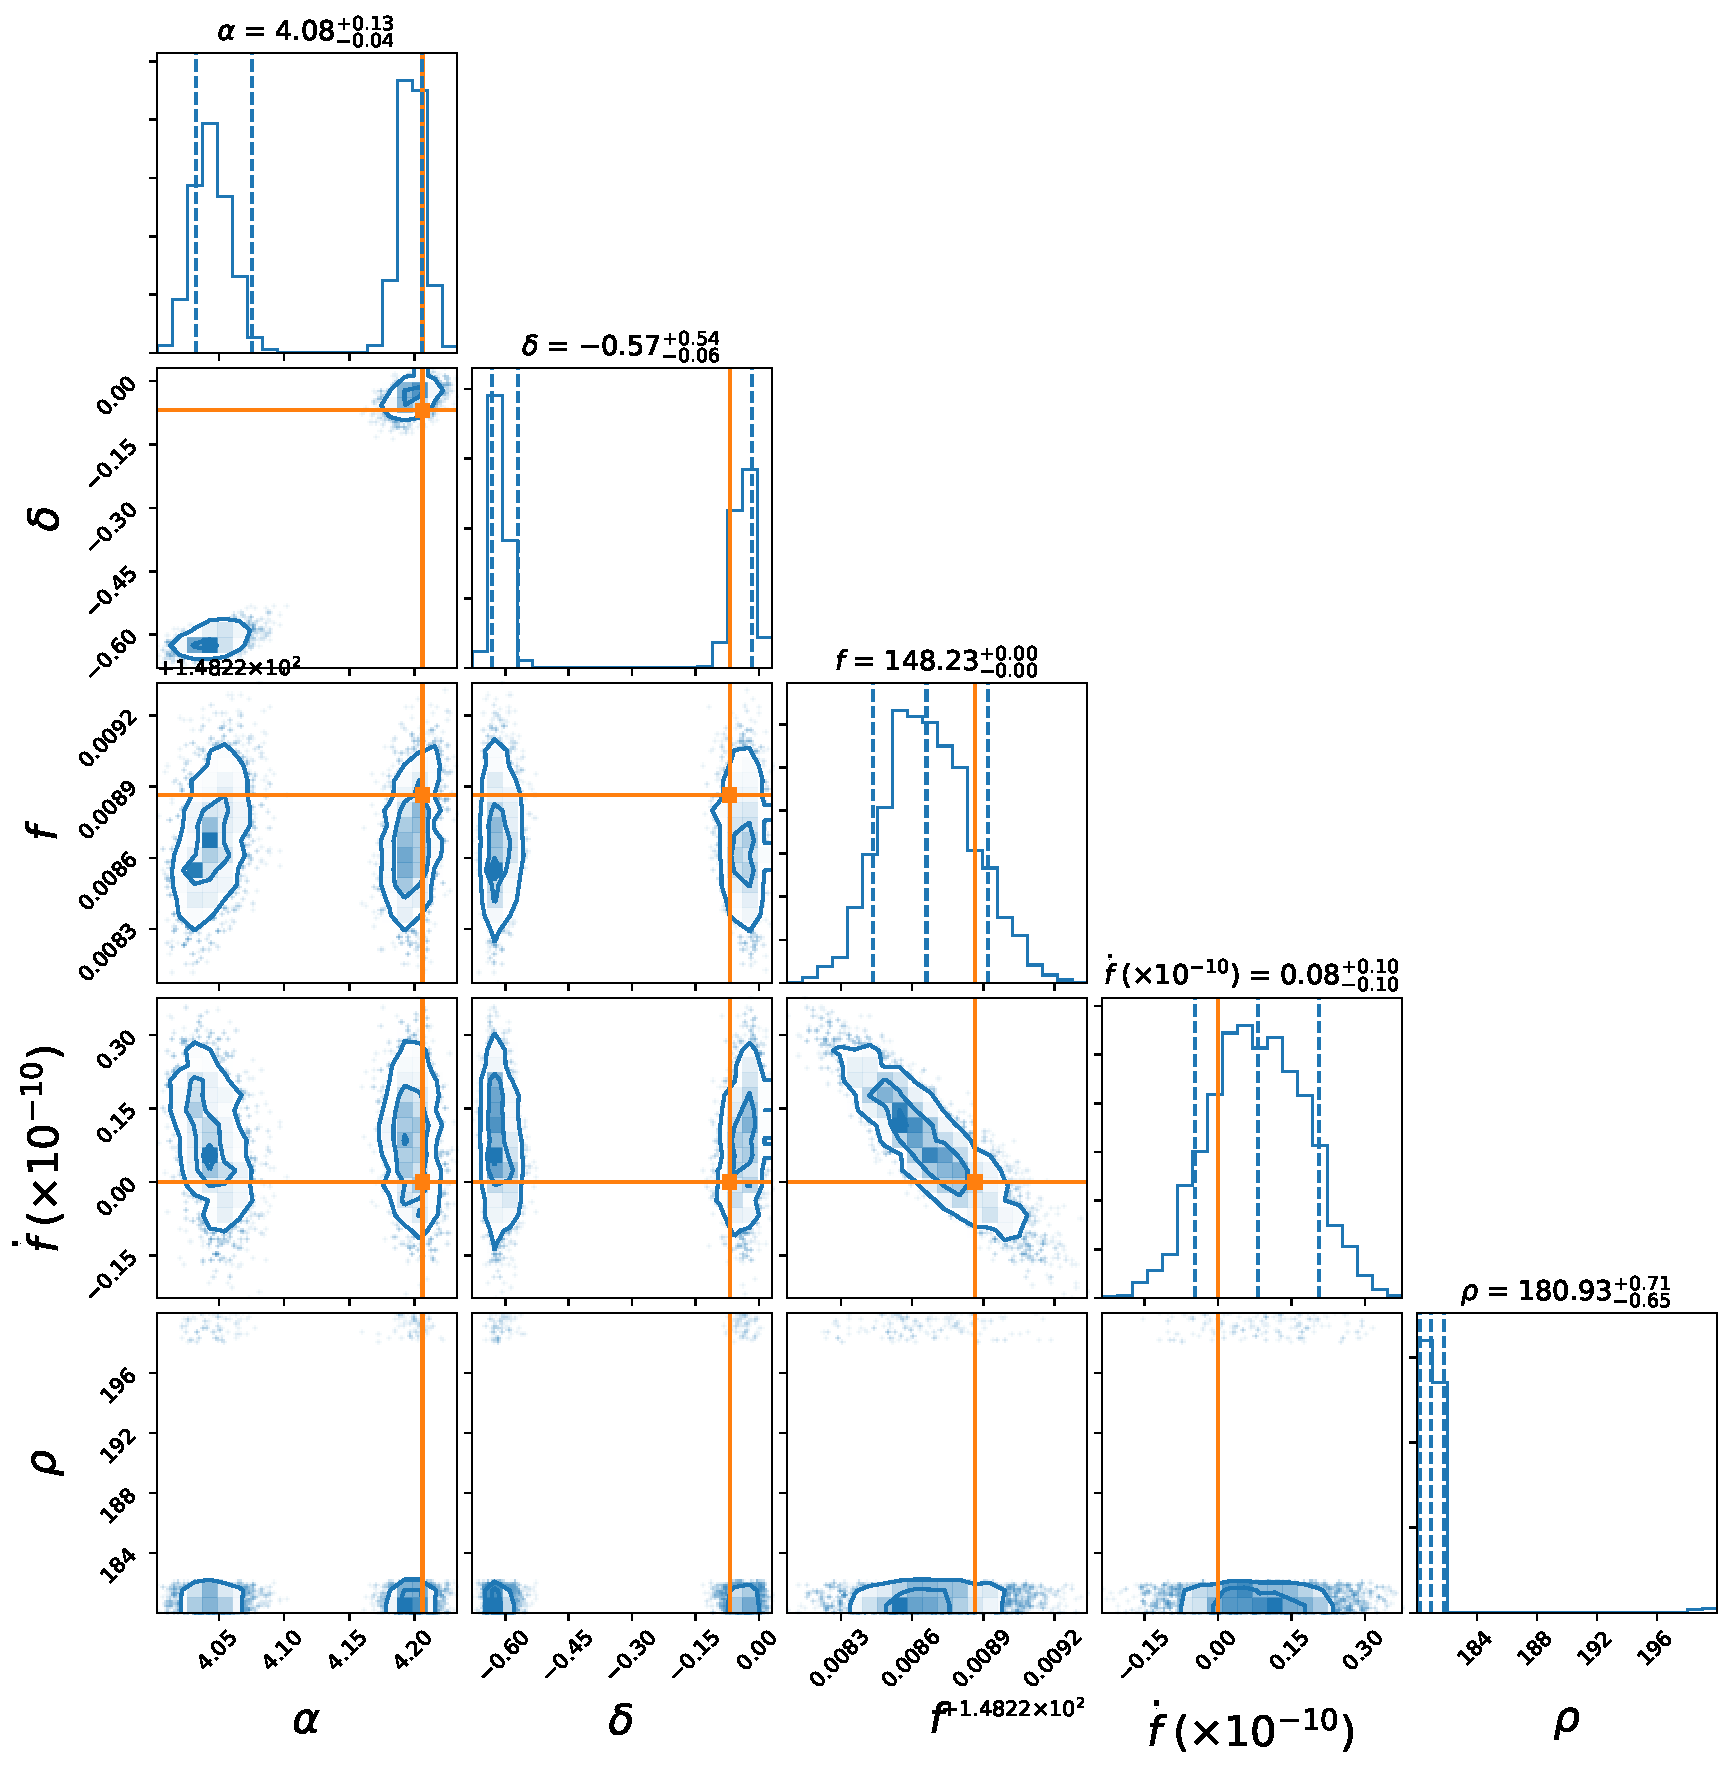
\includegraphics[width=\linewidth]{C5_parameter/cornerplot.pdf}
    \caption[KDE of likelihood in different \gls{SNR} ranges]{This figure shows
an example of the posterior distribution of a signal with \gls{SNR} 151. Each
panel shows the marginal distributions for each parameter, where the parameters
used for the simulation are marked in orange. In this example each of the
posteriors match well with the injected parameters.
The contours on each of the marginal distributions are at confidence levels of 10,50 and 90 \%.}
\label{par_est:results:example_posterior}    
\end{figure}
%

The marginal posterior distribution of the sky parameters is easier to
interpret when it is projected onto a sky map, therefore,
in Fig.~\ref{par_est:results:example_skypos} the parameters $\alpha$ and $\delta$
are shown on a sky projection in the ecliptic frame. The sky
position parameters $\alpha,\delta$ of the \gls{CW} signal are in the
equatorial coordinate system, therefore these have been transformed into the
ecliptic frame $\beta,\gamma$. The Viterbi tracks and \gls{CW} frequency tracks used in this
analysis are sampled once a day, therefore, we should only see the Doppler
modulation from the orbit of the earth around the sun.  In the ecliptic frame,
i.e. where the $z$ axis is perpendicular to the orbital plane of the earth, for
any ecliptic longitude, there are two sky positions at opposite ecliptic
latitudes which will return the same frequency track.  This then means that we
would expect the marginal posterior distribution to have two modes on the sky
at these two locations, where this is seen in
\ref{par_est:results:example_skypos}.
%
\begin{figure}[ht]
    \centering
    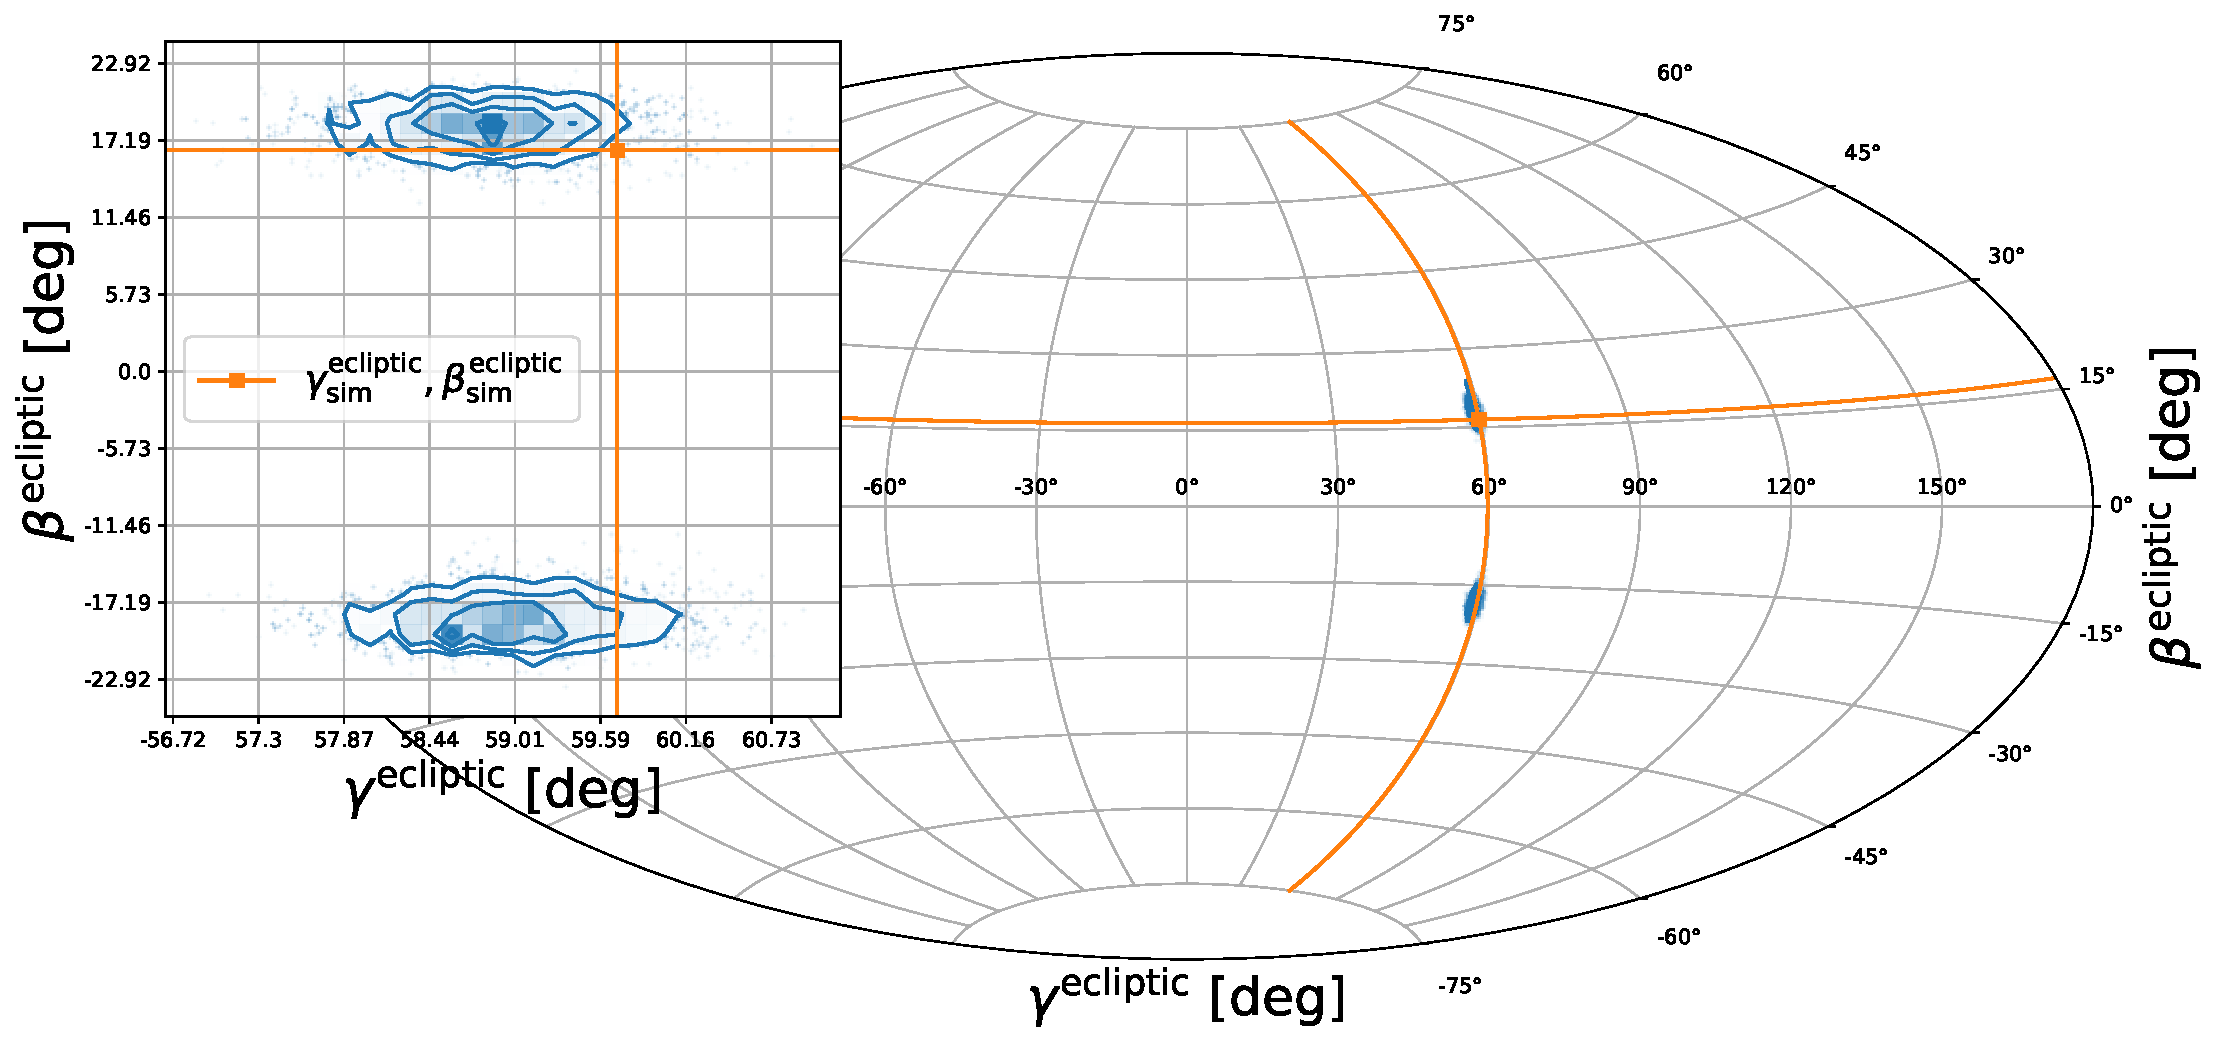
\includegraphics[width=\linewidth]{C5_parameter/skypos_ecliptic.pdf}
    \caption[Example of posterior of sky position in ecliptic frame]{This
figure shows an example of the marginal posterior distribution of the sky
position in the ecliptic frame
$\gamma, \beta$ of a signal with \gls{SNR} 151. The
overlaid panel is a zoomed area around the posterior distribution, where the
orange marker shows the injected parameters. The contours in are defined at 10, 50 and 90 \% confidence.} \label{par_est:results:example_skypos}   
\end{figure}
%

%
%
\subsection{\label{par_est:results:simulations}Simulations}
%
%
To test the Bayesian method described in Sec.~\ref{par_est:bayes}, we generate a
set of spectrograms which contain simulations of \gls{CW} signals in Gaussian noise as in Sec.~\ref{soap:results} and
Sec.~\ref{machine:results}.  This is the same simulated test set from
Sec.~\ref{machine:results}, where \gls{CW} signals were injected into 50\% of
the 0.1 Hz wide sub-bands between between 40 and 500 Hz, with the parameters as
described in Tab.~\ref{machine:data:injections:table}.  The SOAP search using
the line aware statistic with parameters in Tab.~\ref{soap:results:parameters}
is run on each sub-band, where the Viterbi track and \gls{CW} signal parameters
$\alpha, \delta, f, \dot{f}$ and $\rho$ associated with each
simulation are recorded.  The Viterbi track can then be used to run the
Bayesian analysis described in Sec.~\ref{par_est:bayes}.  In these simulations,
we have 2300 simulated signals which have an \gls{SNR} range between 40 and
200, where for this test we randomly select 200 of these simulations.

\if
However, as the \gls{SNR} of the simulations decreases, the probability of SOAP identifying the signal decreases, therefore, we only want to run the Bayesian parameter estimation on signals which are most likely to be astrophysical.
Therefore, as in Sec.~\ref{soap:results}, we find the false alarm rate, which is the fraction of bands which contain no injection and has a Viterbi statistic which exceeds a given threshold, where this is set to 0\% for this test.
We can then select all of the sub-bands which have a Viterbi statistic above this threshold for further investigation, where with a 0\% false alarm rate we have 2000 \joe{ecaxt number} injections to investigate.
The Viterbi statistics for each of these injections can be seen in Fig.~\ref{par_est:results:all_viterbi}, where the 0\% false alarm value is marked.
%
\begin{figure}
    \centering
    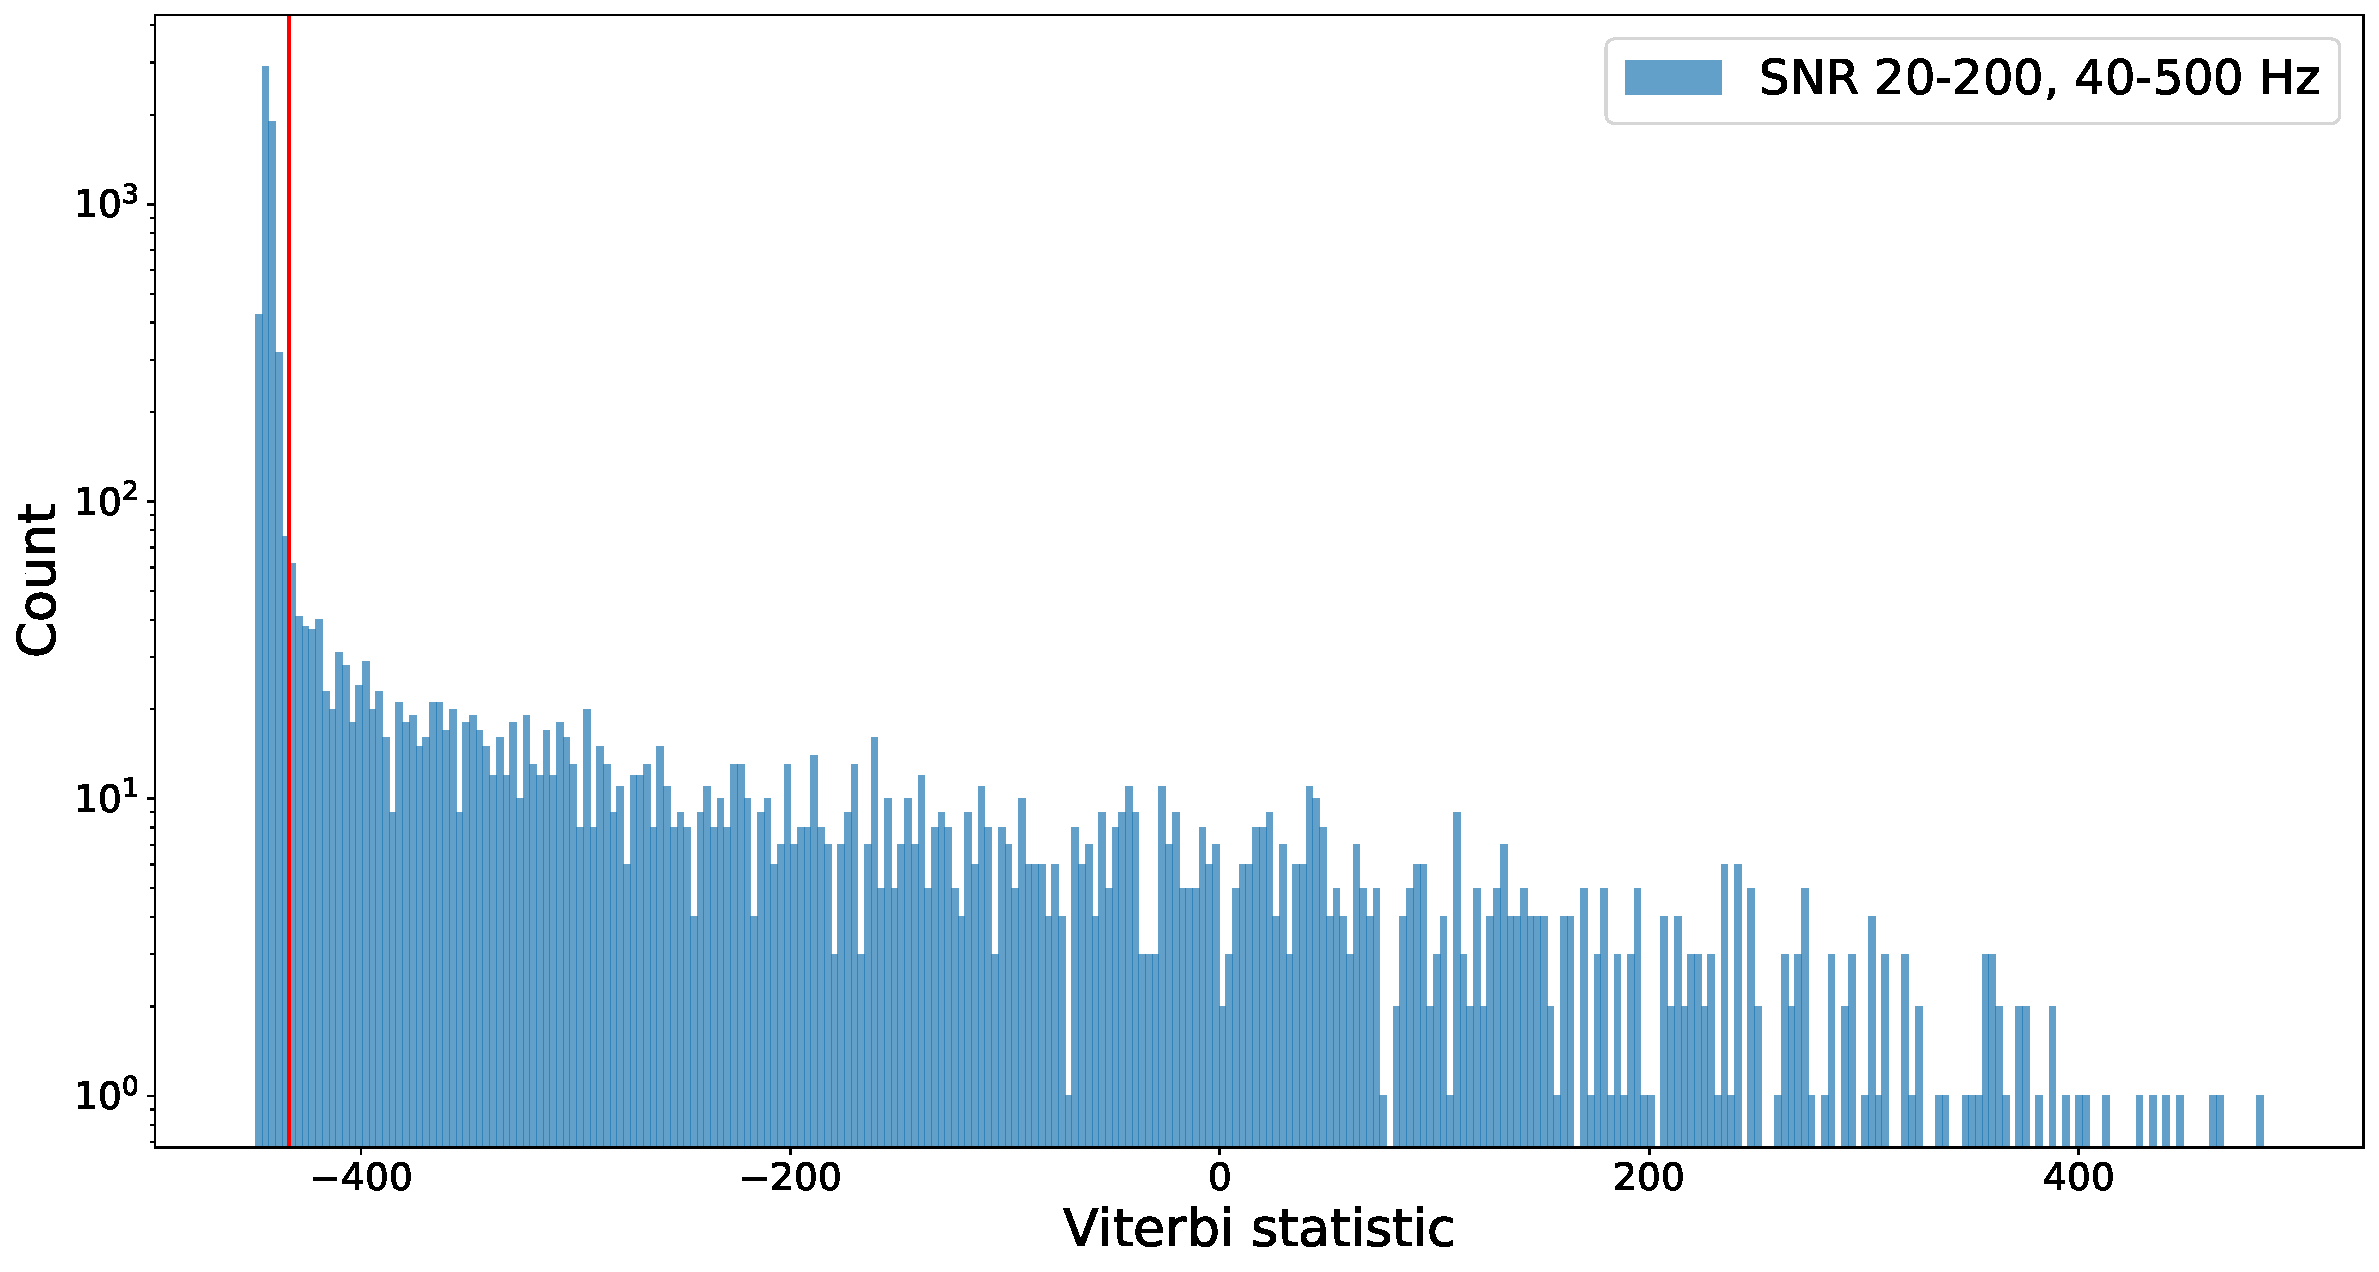
\includegraphics[width=\linewidth]{C5_parameter/viterbi_hist.pdf}
    \caption[All Viterbi statistics]{This figure shows a histogram of the Viterbi statistics from each of the 0.1 Hz wide sub bands in this test. \joe{more}}
    \label{par_est:results:all_viterbi}
\end{figure}
\fi


\subsubsection{\label{par_est:results:simulations:ppplot}$p$--$p$ plot}

The $p$--$p$ plot is a
mechanism to validate the effectiveness of the Bayesian model and computation
using many simulations.  From Sec.~\ref{par_est:results} we have the output
posterior distribution $p(\bm{\theta} \mid \bm{V}, I)$, or more correctly we
have $N$ samples from this distribution $\bm{\theta}_i$, and we have the
injected parameters $\bm{\theta}_{\rm{inj}}$.  For each simulation, we can
calculate the posterior quantile $q(\theta_{\rm{inj}})$ from the marginal
posterior distribution
%
\begin{equation}
    q(\theta_{\rm{inj}}) = P(\theta_{\rm{inj}} > \theta) = \frac{1}{N} \sum_{i=1}^{N} H(\theta_{\rm{inj}} - \theta_i),
\end{equation}
%
where $H(x)$ is the Heaviside step function.  This calculates the fraction of
the marginal posterior distribution which has a parameter $\theta$ less than
the injected parameter $\theta_{\rm{inj}}$ \citep{cook2006ValidationSoftware}.
If the Bayesian model and computation of the posterior is valid, then as the
number of samples approaches infinity ($N \rightarrow \infty$), the posterior
quantile $q(\theta_{\rm{inj}})$ should follow a uniform distribution $[0,1]$
\citep{cook2006ValidationSoftware}.  This then provides a method to check the
validity of our analysis.

For each of our simulations we can calculate $q(\theta_{\rm{inj}})$, such that
we have values $\bm{q}_{\theta}$, where the fraction of simulations which fall
within a given \gls{CI} $C$ is the cumulative distribution of
$\bm{q}_{\theta}$, i.e. $P(\bm{q}_{\theta} > C)$, where $C$ ranges between
$[0,1]$.  If $q(\theta_{\rm{inj}})$ and therefore $\bm{q}_{\theta}$ follows a
uniform distribution, then $P(\bm{q}_{\theta} > C) = C$ \citep{cook2006ValidationSoftware}.
Plotting $P(\bm{q}_{\theta} > C)$ against $C$ for each parameter $\theta$, then
shows the fraction of simulations which have a $q(\theta_{\rm{inj}})$ within
some \gls{CI} $C$, this is known as a $p$--$p$ plot.

If the Bayesian posteriors can be trusted, then this plot should follow a straight
diagonal line, indicated by the black line in
Fig.~\ref{par_est:results:ppplot_example}.  If the the majority of the marginal posterior
distributions are shifted to right of the injected parameters, i.e. the true value lies in
the lower tail of the posterior for the majority of the simulations, then the $p$--$p$ plot will show a curve above
the diagonal, this is shown in the top left
panel of Fig.~\ref{par_est:results:ppplot_example}.  Similarly, if the majority of the marginal posterior distributions are shifted to
left of the injected parameters, i.e. the true value
lies in the upper tail of the posterior for the majority of the simulations,
then the $p$--$p$ plot will show a curve below the diagonal, this is shown in the
top right panel of Fig.~\ref{par_est:results:ppplot_example}.  If the posterior is
under-constrained, i.e. the injected parameters are scattered with a larger width than the posterior suggests, then the curve will follow an S shape
where the S is below the diagonal at $C < 0$.5 and above the diagonal at $C >
0.5$. This is shown in the third panel of
Fig.~\ref{par_est:results:ppplot_example}.  Similarly, if the posterior is over-constrained, i.e. the injected parameters have a narrower distribution than the posterior suggests,, then the curve will follow an S shape where the S is
above the diagonal at $C < 0.5$ and below the diagonal at $C> 0.5$.
%
\begin{figure}[ht]
    \centering
    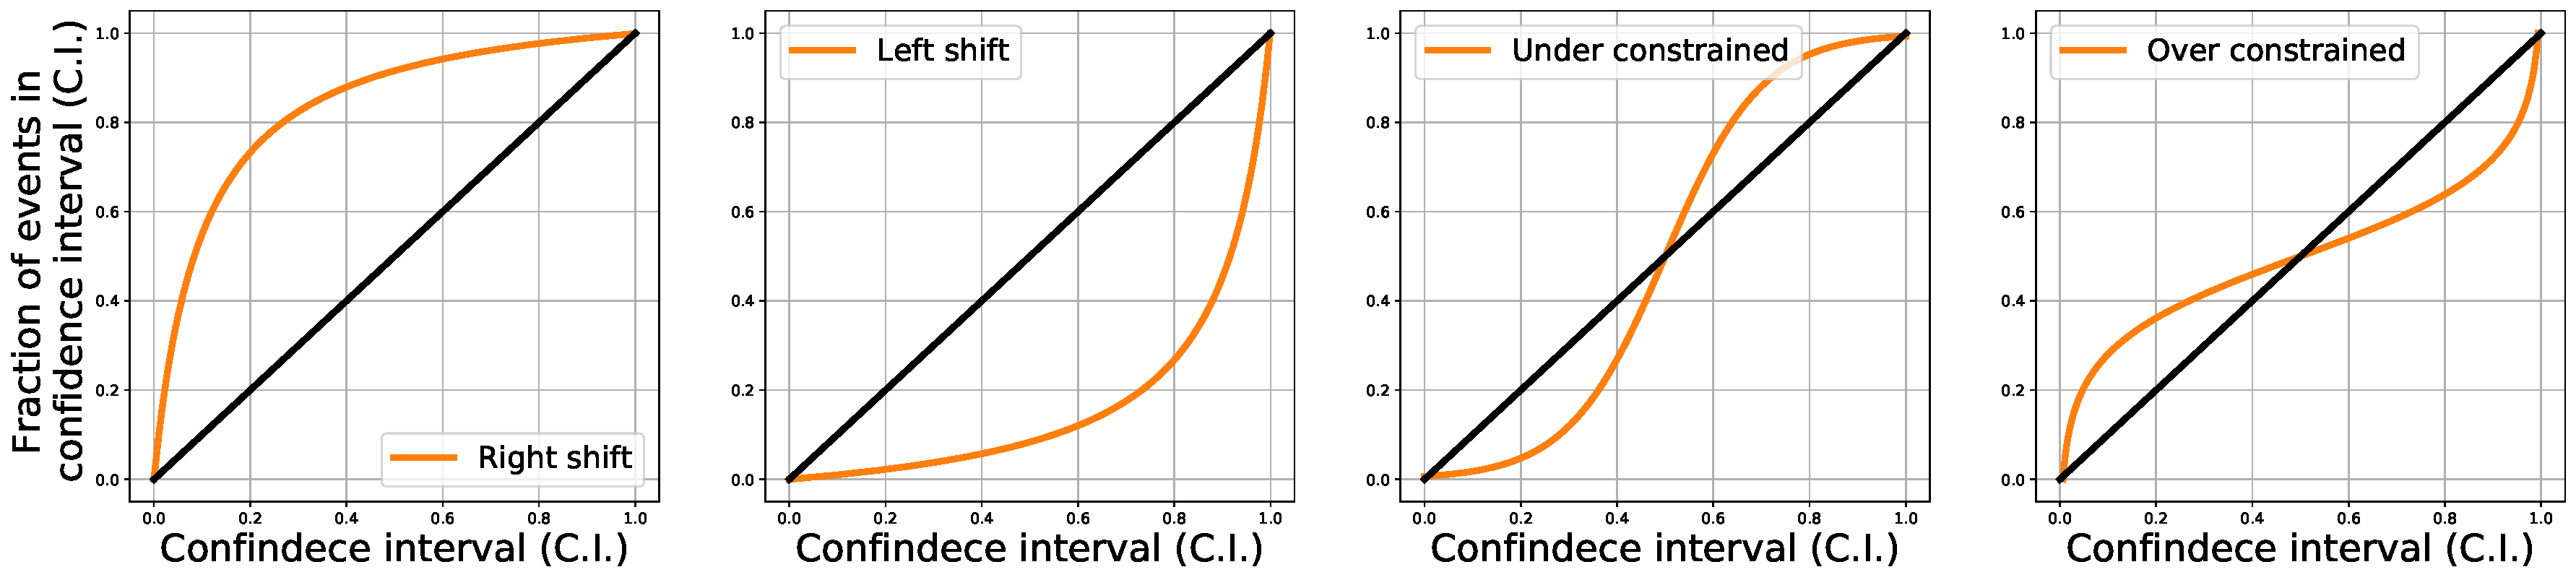
\includegraphics[width=0.9\linewidth]{C5_parameter/ppplot_examples.pdf}
    \caption[$p$--$p$ plot examples]{This figure shows examples of p-p plots for
posterior distributions which are shifted to the right (larger values of the
parameter), to the left (smaller values of the parameter) and over and under
constrained posteriors. The black curve shows the p-p plot when the posterior
distribution is perfectly recovered, i.e. the confidence intervals follow a
uniform distribution.}
\label{par_est:results:ppplot_example}
\end{figure}

We can then generate the $p$--$p$ plot for the 200 simulations in the test described in Sec.~\ref{par_est:results:simulations}, this shown
in Fig.~\ref{par_est:results:ppplot}.  Using the information from Fig.~\ref{par_est:results:ppplot_example}, we can see that for the parameters $f$
and $\dot{f}$ we recover an over-constrained posterior
distribution.  For the \gls{SNR} parameter $\rho$, the recovered posterior is
both shifted to the right and is over constrained, i.e. we assume higher
\glspl{SNR} than perfectly recovered distribution.  For both the right
ascension parameter $\alpha$ and the declination parameter $\delta$, we can see
that we recover an over-constrained posterior distribution at 95\% confidence.  

%
\begin{figure}[ht]
    \centering
    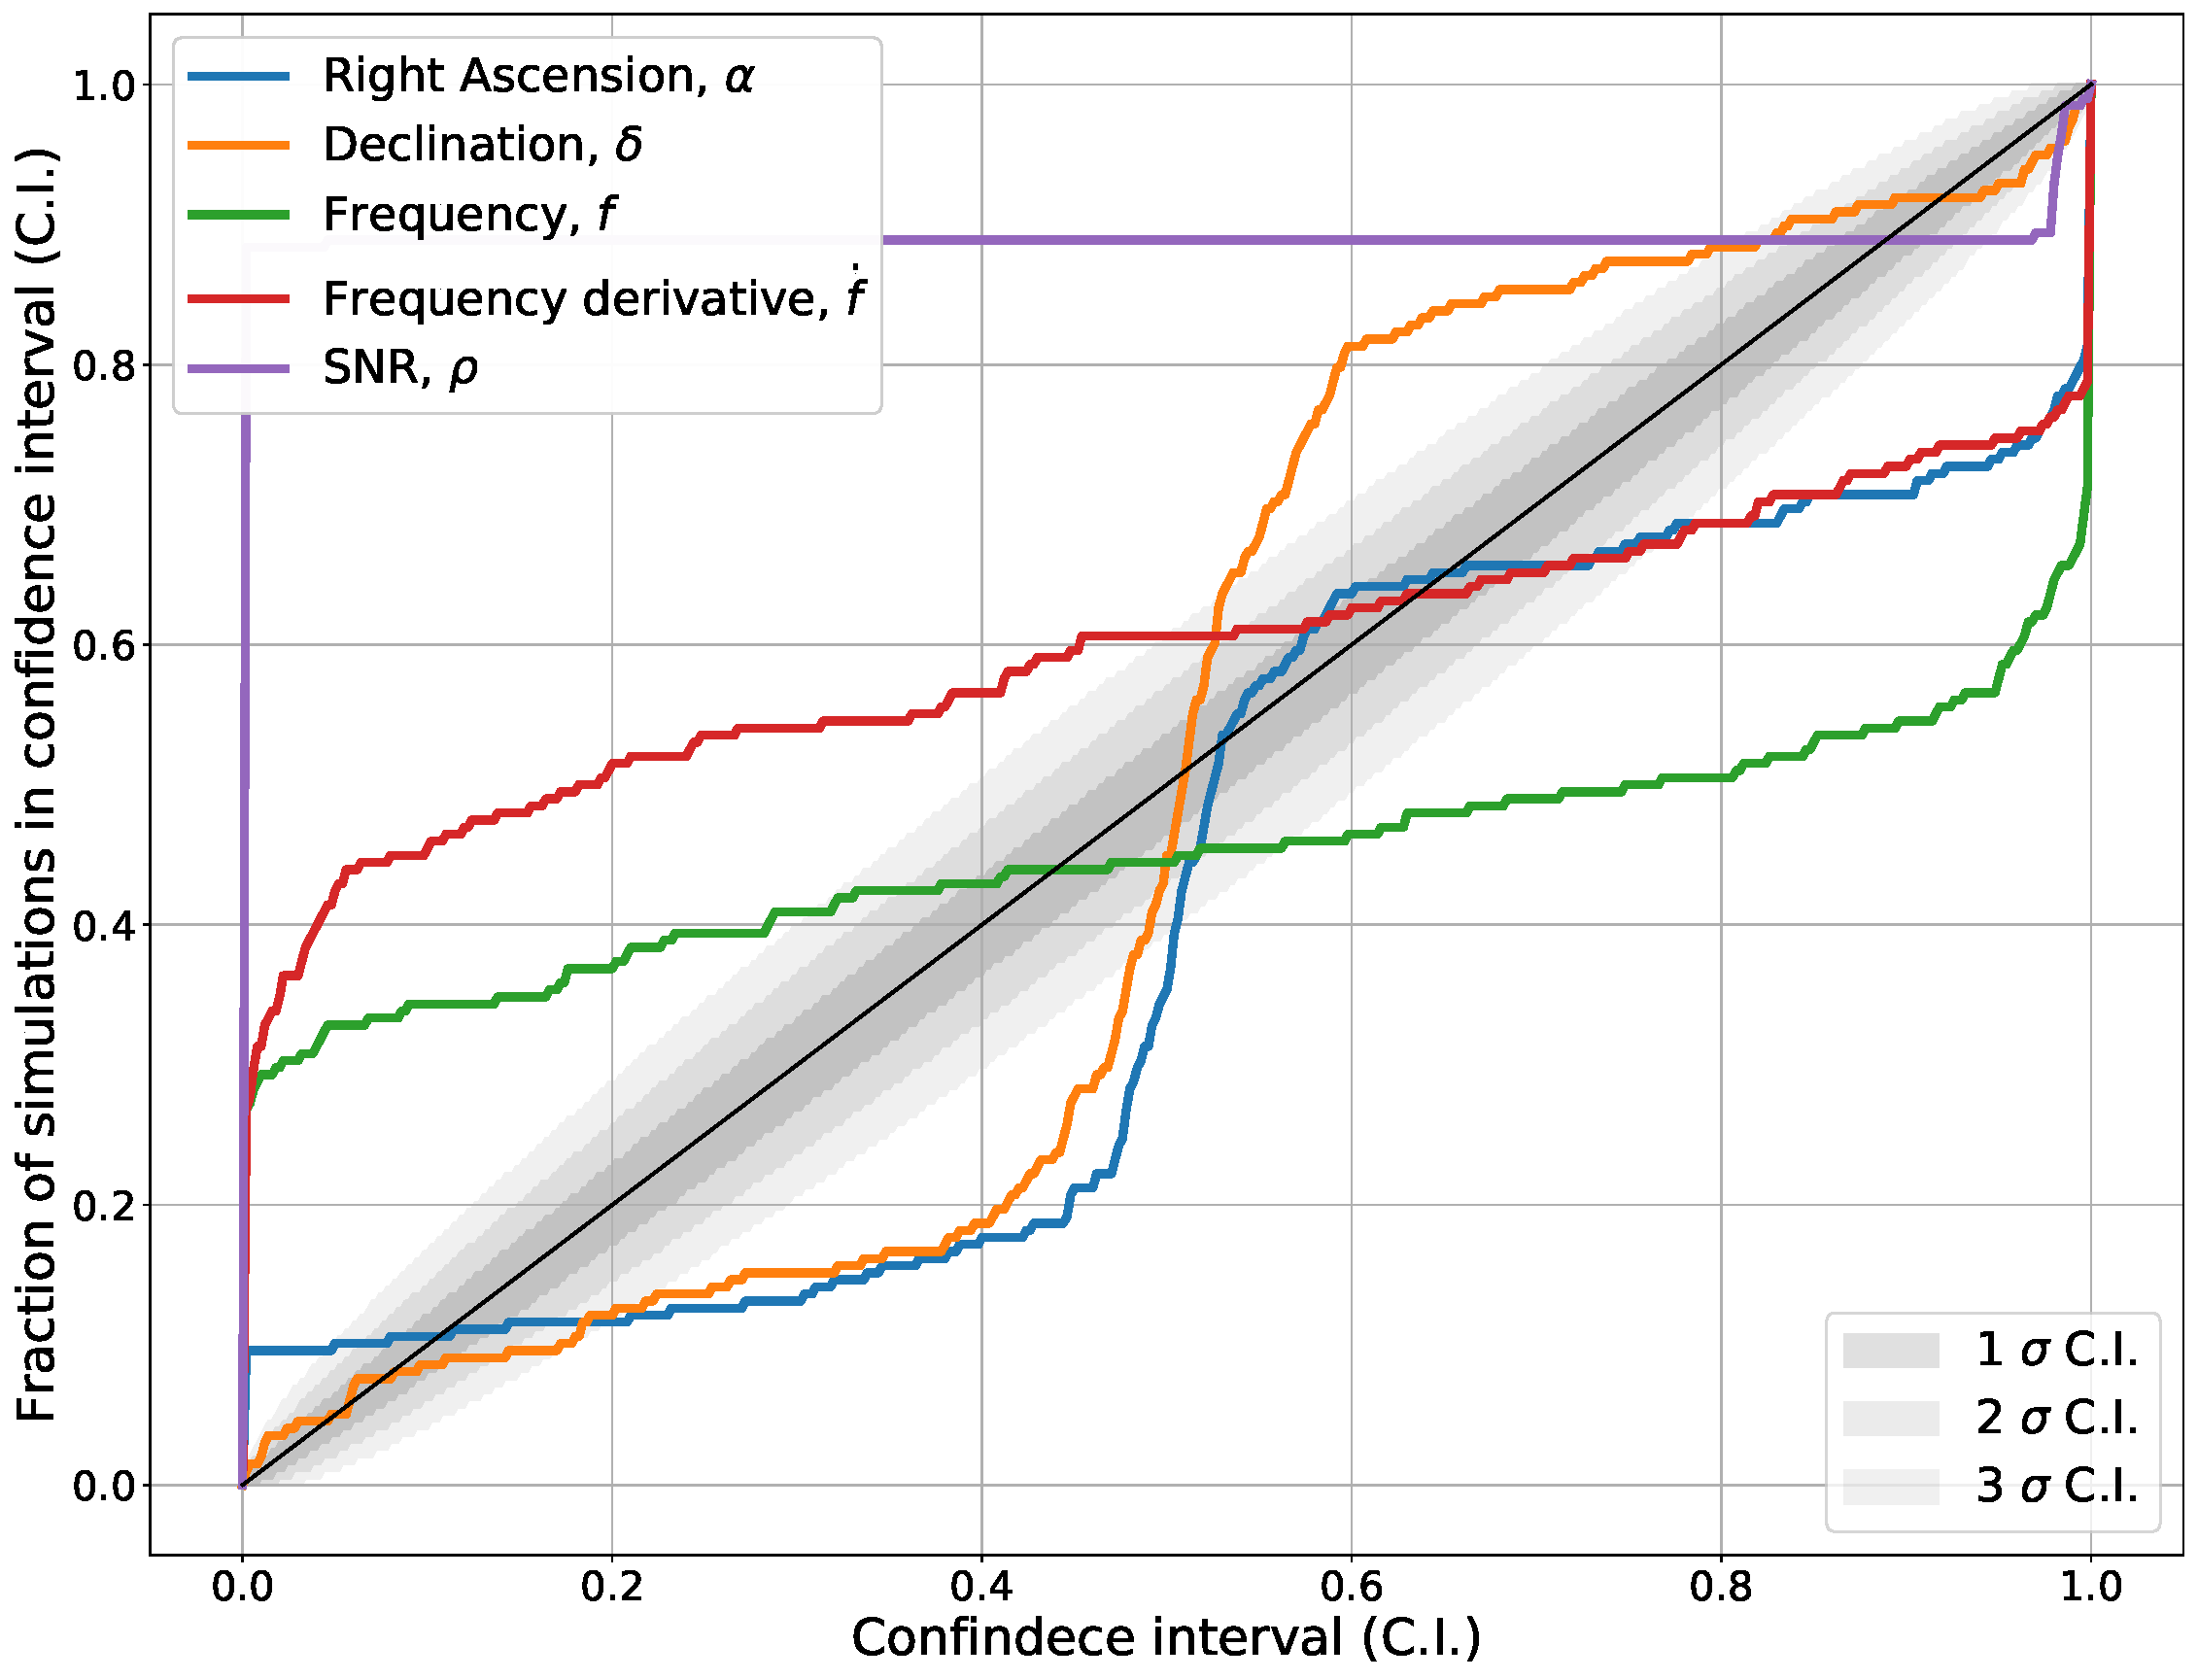
\includegraphics[width=\linewidth]{C5_parameter/ppplot.pdf}
    \caption[p-p plot for the CW simulations]{The p-p plot is shown for the 200
signals described in Sec.~\ref{par_est:results}, which range between 40 and 200
in \gls{SNR}. This describes how well the marginal posterior distributions for
each parameter match the simulated parameter. The \gls{SNR}, frequency and
frequency derivative are over-constrained distributions and the sky position parameters
$\alpha,\delta$ are under-constrained.} \label{par_est:results:ppplot}
\end{figure}

Each of the curves in Fig.~\ref{par_est:results:ppplot} indicate that the
current analysis does not correctly reproduce the true posterior distribution.
One likely reason for this could be due to an incorrect definition of the likelihood in Sec.~\ref{par_est:bayes:likelihood}, for example, to simplify the problem we assume
that all track components are independent, this is not necessarily true and
could contribute to the over constrained posterior
distributions.

%
%
\subsubsection{\label{par_est:results:simulations:skyarea}Sky area at given confidence interval}
%
%

If we assume that the posterior contours are trustworthy, i.e. we do not under constrain or
shift out posterior, then we can estimate the area of the sky which this method can
localise the source to.  To do this we can use our estimation of the marginal
posterior distribution on the sky, and draw a contour on the posterior which
contains 95\% of the probability.  The area contained within this contour is
then the sky area which the source can be localised to at a 95\% confidence,
this can be seen as the green contour in
Fig.~\ref{par_est:results:sky_area_example}.  Similarly, a contour can be drawn
at the values of the injected sky position parameters, this is shown as the red contour in
Fig.~\ref{par_est:results:sky_area_example}. 
This contour defines the confidence at which the injected parameter in contained.

If the contour at the injected parameter is much larger than the contour at 95\%
confidence, then this implies that the posterior distribution is over-constrained.  These two areas are another measure of the validity and ability of this
method to extract the sky parameters. 
%
\begin{figure}[ht]
    \centering
    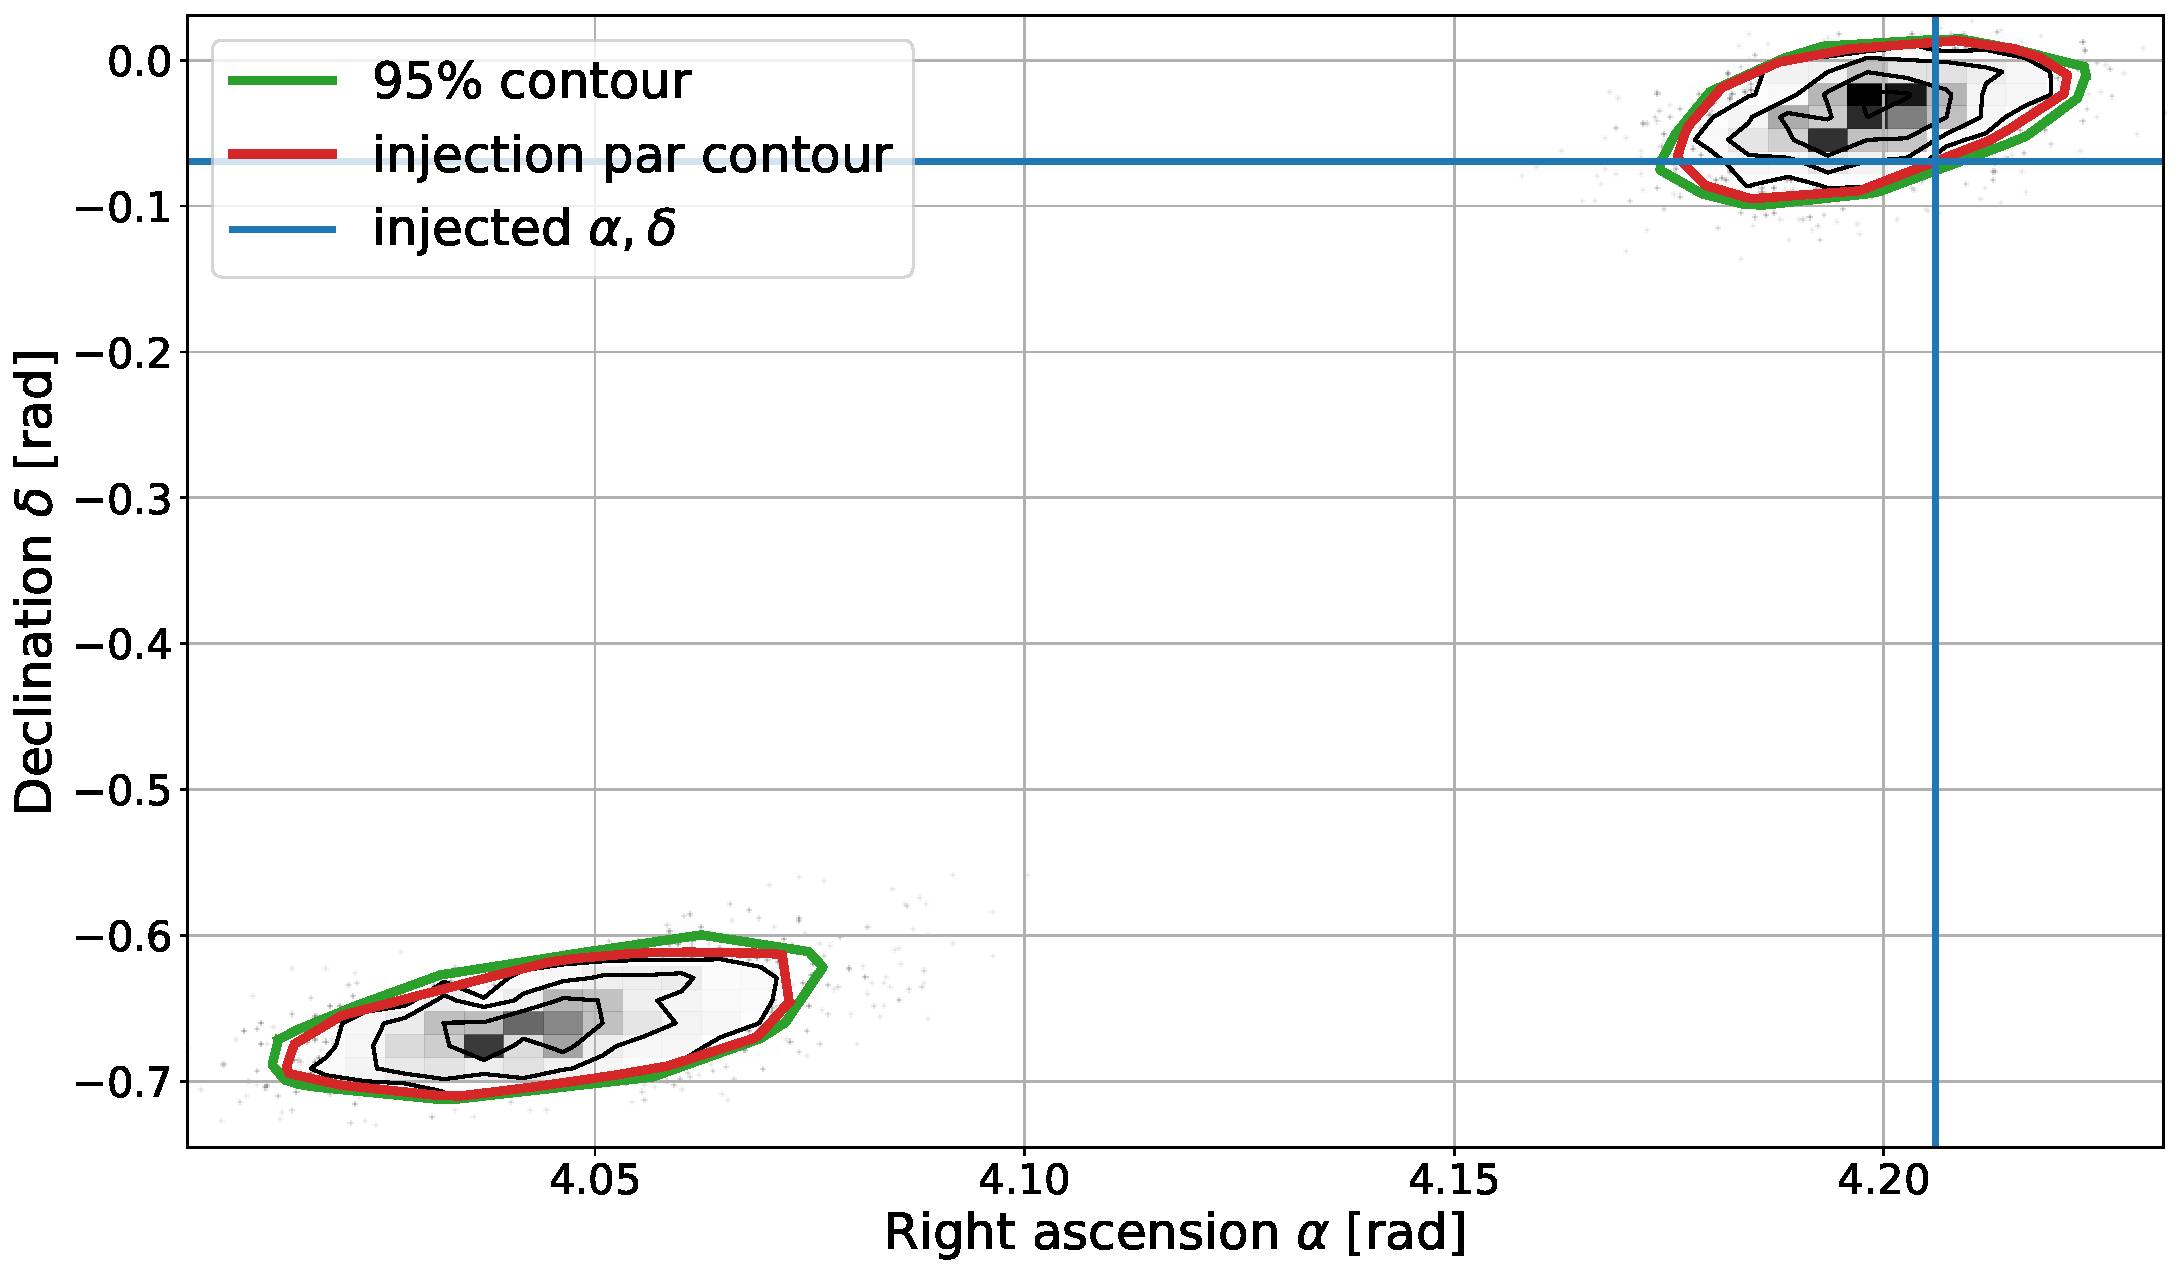
\includegraphics[width=\linewidth]{C5_parameter/skyarea_example.pdf}
    \caption[Area of sky at 95\% confidence]{For the injection in
Sec.~\ref{par_est:results:example_posterior}, the contour in sky position
posterior is drawn for a 95\% confidence and the area which contains the
injected sky position parameters. In this example the two contours are
similar.} \label{par_est:results:sky_area_example}
\end{figure}

The contours and therefore their associated sky areas can be calculated for all
of the simulations described in Sec.~\ref{par_est:results}. The first panel of Fig.~\ref{par_est:results:sky_area} shows the histograms of the areas contained within the contours at 95\% confidence. The second panel shows the areas contained within the contours which are drawn at the value of the injected parameters.
%
\begin{figure}[ht]
    \centering
    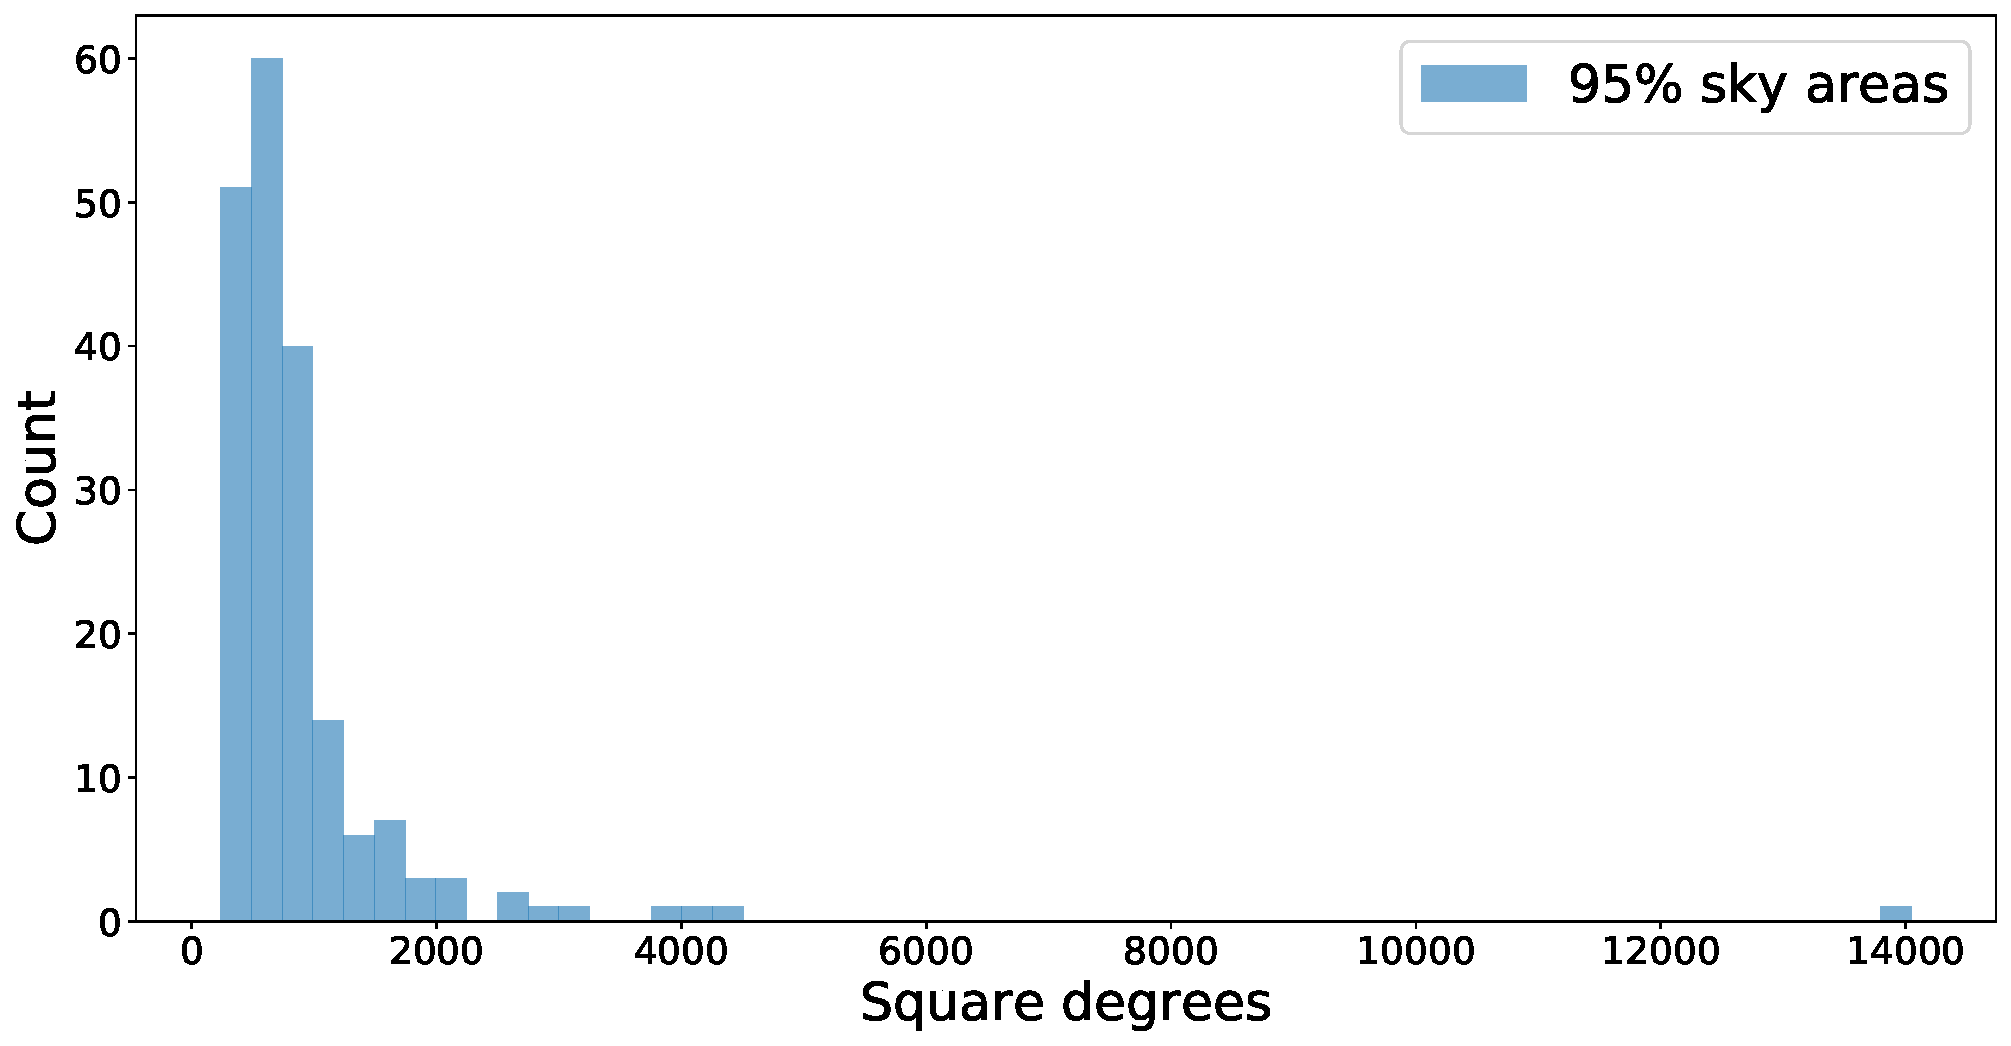
\includegraphics[width=\linewidth]{C5_parameter/sky_area_hist.pdf}
    \caption[histogram showing the area contained within 90\% confidence contours]{
    	The top panel shows a histogram of the sky area which this method can localise a source to with 95\% confidence. This is the area of a contour which contains 95\% of the posterior distribution.
    	The second panel shows the sky areas associated with a contour which is draw on the posterior through the injected parameter value. 
    	From the first panel, we can say that 90\% of the time we can localise to a sky area less than 45 deg$^2$ with 95\% confidence, this is shown as the red 90\% confidence line in both panels.
    	The true parameter however, is contained within the 95\% contour only 23\% of the time.}
\label{par_est:results:sky_area} 
\end{figure}
%
From the distributions in Fig.~\ref{par_est:results:sky_area} we can see that
the sky areas which contain the injected parameters are larger by a factor of
$\sim 10$ than those at 95\% confidence.  We can also determine from this that the injected
parameters fall within the 95\% confidence contour only 23\% of the time.  This
implies that these posterior distributions are over-constrained, and that the sky areas at 95\% confidence is overly optimistic.

However, if we assume that the 95\% confidence sky areas are trustworthy, we can approximate the sky area which this method can localise to. 
From the first panel in Fig.~\ref{par_est:results:sky_area}, we can say that 90\% of the time we can localise to a sky area
less than 45 deg$^2$ with 95\% confidence. In this case the sky area only contains the true parameter 23\% of the time. 
However, if we did trust the value of 45 deg$^2$, given the
full sky has $\sim 41253$ square degrees, this is factor of $\sim 10^{-3}$ of
the whole sky.  For a fully coherent search for \gls{CW}, this reduction in sky area would
drastically reduce the computational cost of the of the search.


%
%
\section{Discussion}
%
%

In this chapter we describe a Bayesian
analysis to extract the Doppler parameters $\alpha, \delta, f \dot{f}$ and
\gls{SNR} $\rho$ of a potential \gls{CW} source from the Viterbi track which is
described in the SOAP search in Chapter \ref{soap}. The aim of
this method is to provide estimates of the \gls{CW} parameters, and then use
these to reduce the size of the parameter space for a more sensitive fully coherent search. 

In Sec.~\ref{par_est:bayes} we outline the setup of a Bayesian model,
where the input is a Viterbi track which is described in Chapter \ref{soap}, and the output is a posterior distribution of
the Doppler parameters of a \gls{CW} signal.  In this model, the likelihood is
empirically calculated by simulating $\mathcal{O}(10^4)$ \gls{CW} signals and
then recording the difference between the Viterbi track and \gls{CW} frequency
track for multiple \gls{SNR} bands.  The histogram of these values is
then used to construct the likelihood of this method.  For each of the
parameters in the search, we assume a flat prior.  In
Sec.~\ref{par_est:results}, the analysis is tested on 200 simulations which had
parameters drawn from the same prior as the Bayesian model.  In this section we
generate p-p plots to asses the validity of this model and find that the
\gls{SNR}, frequency and frequency derivative all are over constrained
distributions and the sky position parameters are a mixture of over and under-constrained depending on the confidence. 

We investigated the area contained within contours on the marginal posterior
for the sky position to gauge the ability of the search to localise a source,
where we found that with a 95\% confidence we can detect to a sky area within
45 deg$^2$ 90\% of the time.  
However, the true value of the parameter fell within this contour only 23\% of the
time, implying that the posterior distributions are over-constrained.
To contain the true value 95\% of the time, this sky area would have to be expanded by a factor of $\sim 30$.
Other methods could be used to reduce this sky area such as using the antenna response of the detector, this would locate the source to one hemisphere removing one mode from the bi modal sky distribution.

These results imply that in its current state, the search does not provide a
valid way to estimate the parameters of the source from its Viterbi track.
However, this is a toy case and with the development of a more appropriate likelihood function and
further investigation, we aim to develop this such that it can correctly
estimate \gls{CW} parameters.



















